\documentclass{report}

\usepackage{amsmath}
\usepackage{amssymb}
\usepackage{amsthm}
\usepackage{tikz}
\usetikzlibrary{positioning}
\usetikzlibrary{automata}

\newtheorem{theorem}{Theorem}[chapter]
\newtheoremstyle{exampstyle}
  {\topsep} % Space above
  {\topsep} % Space below
  {} % Body font
  {} % Indent amount
  {\bfseries} % Theorem head font
  {.} % Punctuation after theorem head
  {.5em} % Space after theorem head
  {} % Theorem head spec (can be left empty, meaning `normal')
\theoremstyle{exampstyle} \newtheorem{example}[theorem]{Example}
\theoremstyle{exampstyle} \newtheorem{remark}[theorem]{Remark}
\theoremstyle{exampstyle} \newtheorem{definition}[theorem]{Definition}
\theoremstyle{exampstyle} \newtheorem{lemma}[theorem]{Lemma}
\theoremstyle{exampstyle} \newtheorem{proposition}[theorem]{Proposition}

\usepackage[english]{babel}
\usepackage{csquotes}
\usepackage{graphicx}
\usepackage{verbatim}
\usepackage{listings}
\usepackage{float}
\usepackage{dsfont}
\usepackage[width=6in, height=8in]{geometry}
%\usepackage{geometry}
\usepackage{xcolor}

\usepackage[
backend=biber,
natbib=true,
url=true, 
doi=true,
eprint=true
]{biblatex}
\addbibresource{sources.bib}


% agsm is harvard
% unsrt is standard numerical
% ieeetr is whatever jasmine uses

\definecolor{codegreen}{rgb}{0,0.6,0}
\definecolor{codegray}{rgb}{0.5,0.5,0.5}
\definecolor{codepurple}{rgb}{0.58,0,0.82}
\definecolor{backcolour}{rgb}{0.95,0.95,0.92}

\lstdefinestyle{mystyle}{
	backgroundcolor=\color{backcolour},   
	commentstyle=\color{codegreen},
	keywordstyle=\color{magenta},
	numberstyle=\tiny\color{codegray},
	stringstyle=\color{codepurple},
	basicstyle=\ttfamily\footnotesize,
	breakatwhitespace=false,         
	breaklines=true,                 
	captionpos=b,                    
	keepspaces=true,                 
	numbers=left,                    
	numbersep=5pt,                  
	showspaces=false,                
	showstringspaces=false,
	showtabs=false,                  
	tabsize=2
}

\lstset{style=mystyle}

\setcounter{tocdepth}{1}

\begin{document}

\begin{titlepage}
    \begin{center}
        \vspace*{1cm}
            
        \Huge
        \textbf{Geometric Numerical Integration}
            
        \vspace{0.5cm}
        \LARGE
        Numerical Methods for Structural Preservation of Ordinary Differential Equations
            
        \vspace{1.5cm}
            
        \textbf{Will Woolfenden}
        
        \vspace{0.5cm}
        
        $10628968$
            
        \vfill

        Project supervisor: Dr. Marcus Webb \\

        \vspace{0.8cm}
            %final submission
        Submission for MATH40000 Double Project for the $2023/24$ academic year
            
        \vspace{0.8cm}
            
        \Large
        
        Department of Mathematics \\
        School of Natural Sciences\\
        The University of Manchester\\
        United Kingdom\\
        \today
    \end{center}
\end{titlepage}

\begin{abstract}
    This is very abstract.
\end{abstract}

\tableofcontents

\documentclass{report}

\usepackage{amsmath}
\usepackage{amssymb}
\usepackage{amsthm}
\usepackage{tikz}
\usetikzlibrary{positioning}
\usetikzlibrary{automata}


\newtheorem{theorem}{Theorem}[chapter]
\newtheoremstyle{exampstyle}
  {\topsep} % Space above
  {\topsep} % Space below
  {} % Body font
  {} % Indent amount
  {\bfseries} % Theorem head font
  {.} % Punctuation after theorem head
  {.5em} % Space after theorem head
  {} % Theorem head spec (can be left empty, meaning `normal')
\theoremstyle{exampstyle} \newtheorem{example}[theorem]{Example}
\theoremstyle{exampstyle} \newtheorem{remark}[theorem]{Remark}
\theoremstyle{exampstyle} \newtheorem{definition}[theorem]{Definition}
\theoremstyle{exampstyle} \newtheorem{lemma}[theorem]{Lemma}

\usepackage[english]{babel}
\usepackage{csquotes}
\usepackage{graphicx}
\usepackage{verbatim}
\usepackage{listings}
\usepackage{float}
\usepackage{dsfont}
\usepackage[width=6in, height=8in]{geometry}
\usepackage{xcolor}

\usepackage[
backend=biber,
natbib=true,
url=false, 
doi=true,
eprint=false
]{biblatex}
\addbibresource{sources.bib}

\definecolor{codegreen}{rgb}{0,0.6,0}
\definecolor{codegray}{rgb}{0.5,0.5,0.5}
\definecolor{codepurple}{rgb}{0.58,0,0.82}
\definecolor{backcolour}{rgb}{0.95,0.95,0.92}

\lstdefinestyle{mystyle}{
	backgroundcolor=\color{backcolour},   
	commentstyle=\color{codegreen},
	keywordstyle=\color{magenta},
	numberstyle=\tiny\color{codegray},
	stringstyle=\color{codepurple},
	basicstyle=\ttfamily\footnotesize,
	breakatwhitespace=false,         
	breaklines=true,                 
	captionpos=b,                    
	keepspaces=true,                 
	numbers=left,                    
	numbersep=5pt,                  
	showspaces=false,                
	showstringspaces=false,
	showtabs=false,                  
	tabsize=2
}

\lstset{style=mystyle}

\begin{document}

\chapter{Introduction}

\section{Motivation}

The goal of this project is to discuss and analyse methods for the preservation of qualitative behaviour when solving ordinary differential equations using numerical methods.
A system of ordinary differential equations (ODEs) often arises when constructing a mathematical model to describe some sort of system: a set of variables and a description of how they change in time.
In absolute most general form, a system of ODEs has the appearance
\begin{equation}
    \frac{\mathrm{d}x}{\mathrm{d}t} = f(t,x)
\end{equation}
where the left-hand side expresses a change of $x$ in time, while the right-hand side is some arbitrary function on $t$ and $x$.
This is a first-order ODE, but in generality we can use this form to express ODEs of any order by considering the solution to be a vector of variables.
Consider the example second order problem
\begin{equation*}
    \frac{\mathrm{d}^2 x}{\mathrm{d}t^2} = \mathrm{e}^{tx}.
\end{equation*}
In this case, let us write this equation in terms of a vector $\mathbf{x}$ of derivatives:
\begin{equation*}
    \mathbf{x} := \begin{pmatrix}
        x \\
        \dot{x}
    \end{pmatrix}.
\end{equation*}
For compactness, we use the dot notation as a shorthand for a time derivative.
We can write our problem as
\begin{equation*}
    \frac{\mathrm{d}}{\mathrm{d}t} \begin{pmatrix}
        x \\
        \dot{x}
    \end{pmatrix} = \begin{pmatrix}
        \dot{x} \\
        \mathrm{e}^{tx}
    \end{pmatrix}
\end{equation*}
which can be expressed in general as
\begin{equation*}
    \frac{\mathrm{d}\mathbf{x}}{\mathrm{d}t} = F(t,\mathbf{x})
\end{equation*}
where $F$ is an arbitrary function again, by no means linear in $\mathbf{x}$.
This framework is fundamental to the methods we will look into for solving ODEs, hence we introduce it now.
The problems we will look at will involve vector solutions in general, so our notation will usually instead denote the whole vector quantity of interest as $x$,
and make sure to individually distinguish its elements if needed.

Since there is a mixed $tx$ term, this is what we call a nonlinear equation.
This means that we cannot write a solution $x(t)$ in closed form using analytical methods.
Instead, we need to use a numerical method.
A numerical method provides us with a sequence of values $(x_i)_{i=1}^n$ for given points in time $(t_i)_{i=1}^n$, where each $x_i$ is an approximation to the true solution $x_i \approx x(t_i)$.
This is the ``numerical integration'' of this project.
Numerical methods, especially the ones we will look at, are aimed at solving Initial Value Problems (IVPs), where we want to solve the ODE given an initial condition $x(t=0) = x_0$.
Alternatively, a boundary value problem specifies conditions on the boundary of a domain. For example, consider a second order ODE\footnote{
    A problem of order $n$ requires $n$ conditions in order to have a unique solution.
} with constraints at $x(t=0)$ and $x(t = t_n)$.
Numerical methods for boundary value problems are fundamentally different to the methods for initial value problems we will study, hence we will not consider them in this report.

For a first example, we will consider Euler's method. This method starts by assuming a value $x(t_i) = x_i$ and considering the next value.
We denote the \textit{step size} by $h$, being the difference $t_{i+1} - t_i$.
Then we consider the next value by evaluating the Taylor series
\begin{equation*}
    x(t_i + h) = x(t_i) + h \dot{x}(t_i) + \frac{h^2}{2}\ddot{x}(t_i) + \frac{h^3}{6}\dddot{x}(t_i) + \mathellipsis = \sum_{k=0}^{\infty} \frac{h^k x^{(k)}(t_i)}{k!}.
\end{equation*}
On the left-hand side, the next point in time $t_{i+1}$ is the same as $t_i + h$.
On the right-hand side, if we assume $h$ is small then we can simplify this problem by assuming that every term of $h$ of order $2$ or greater is negligibly small.
We write this as $\mathcal{O}(h^2)$. The big-O notation means that as $h \rightarrow 0$, the expression is bounded above by some constant times $h^2$.
The whole equation reduces to
\begin{equation*}
    x(t_{i+1}) = x_i + hf(t_i, x_i) + \mathcal{O}(h^2).
\end{equation*}
We know what $f$ is, since it defines the ODE. We also assumed a value $x_i$ for a value (or approximation) of $x(t_i)$.
If we ignore the $\mathcal{O}(h^2)$ term, we are left with what is generally referred to as the forward Euler method
\begin{equation}
    x_{i+1} = x_i + h f(t_i, x_i)
\end{equation}
for solving an ODE.

One element that we will focus on is the concept of error and accuracy of a numerical method.
It turns out that ignoring the $\mathcal{O}(h^2)$ in order to obtain Euler's method was not a fantastic idea.
Euler's method is what we refer to as first-order accurate.
This means that the expressions for the true solution (by Taylor series) and the approximation (by the method) are the same up to and including the term in $h$ of order $1$.
Here we define the concept of truncation error as $\tau(h) = x(t_i) - x_i$, being the error between the true solution and the approximation for a single step of size $h$.
As we have seen, the local truncation error of Euler's method is $\mathcal{O}(h^2)$.
We also want to consider the concept of global truncation error, which is the error accumulated over an entire numerical solution.
This is important because each step comes from a previous point, and only the initial value is given as exact. % the next bit is VERY HANDWAVY
The local error of Euler's method is $\mathcal{O}(h^2)$, and assume it requires $N$ timesteps in order to compute a numerical solution.
Then the global error is $\mathcal{O}(Nh^2)$. But $N$ is proportional to $1/h$ since $h = (t_n - t_0)/N$, and so the global error is $\mathcal{O}(h)$.
This argument can be generalised to any method with uniform timestep.

The problem of global error analysis arises when considering how we may need a computation to match a certain tolerance.
Assume we need the global error of a numerical solution to be below $\epsilon$.
This means we need the sum of the truncation errors across the whole computation to be below this threshold.
Ignore how we compute or estimate the truncation error, which we will explore later.
Assume we perform a computation and our global error is less than or equal to $8 \epsilon$.
We need to divide the global error by $8$. For a method with global truncation error $\mathcal{O}(h^3)$,
we can half the step size and run the computation again to match this tolerance, since if $C h^3 \approx 8 \epsilon$ then $C (h/2)^3 \approx \epsilon$.
Whereas for a lower order method, this would be much more expensive, perhaps prohibitively more so.

If we want to improve error, we may start by considering a Runge-Kutta method.
These are methods given by
\begin{equation*}
	x_{n+1} = x_n + h \left( \sum_{i = 1}^{s} b_i k_i \right)
\end{equation*}
where the $b_i$ are coefficients and the $k_i$ are ``guesses'' of the form
\begin{equation*}
	k_i = f \left( t_n + c_i h,~ x_n + h\sum_{j = 1}^{s} a_{ij}k_j \right).	
\end{equation*}
By using linear combinations of the $k_i$, we want to reduce the truncation error to a certain order.
For compactness, a Runge-Kutta method is often expressed as its Butcher tableau
\begin{equation*}
	\begin{array}{c|ccc}
		c_1  &a_{11} &\dots &a_{1s} \\
		\vdots &\vdots & &\vdots \\
		c_s &a_{s1} &\dots &a_{ss} \\
		\hline
		&b_1 &\dots &b_s
	\end{array}.
\end{equation*}
Runge-Kutta methods are extremely popular choices for higher order integrators.









\end{document}



\chapter{Symplectic Integration}

\section{Hamiltonian Systems and Numerical Methods}

\subsection{Hamiltonian Dynamics}

A Hamiltonian system on $(q,p)$ is given by
\begin{align*}
	&\dot{q} = \dfrac{\partial H}{\partial p}
	&
	\dot{p} = \dfrac{-\partial H}{\partial q}&.	
\end{align*}
We use $q$ to denote position, and $p$ to denote momentum.
This is a special form of a general system of ODEs $\dot{x} = f(t,x)$.
For this part of our discussion, we will primarily be concerned with \textit{autonomous} systems of the form $\dot{x} = f(x)$.

The Hamiltonian $H(q,p)$ is a first integral of the system, used to denote the total energy.
We can write the system as
\begin{equation}
	\dfrac{\mathrm{d}}{\mathrm{d}t}\begin{pmatrix}
		q \\
		p
	\end{pmatrix} = \begin{bmatrix}
		\strut 0 & \strut 1 \\
		\strut -1 & \strut 0
	\end{bmatrix}\begin{bmatrix}
	\dfrac{\strut \partial H}{\strut\partial q} \\
	\dfrac{\strut \partial H}{\strut\partial p}
	\end{bmatrix}.
\end{equation}
If we write $x = (q,p)^\mathrm{T}$ and denote the matrix as $J$,
then the statement of a Hamiltonian system is of the form 
\begin{equation}
	{\dot{x}} = {J}\nabla H({x}).
	\label{eqn:hdyn}
\end{equation}
We call $J$ the \textit{symplectic matrix}.

For a $d$-dimensional problem,
we instead denote the variables $q_1, \mathellipsis, q_n, p_1, \mathellipsis, p_n$ as the position and momentum in the directions of each basis vector respectively.
Write $x = (q_1, \mathellipsis, q_n, p_1, \mathellipsis, p_n)$.
Define $J$ to be the matrix defined in blocks
\begin{equation}
	J = \begin{bmatrix}
		{0}_n & {I}_n \\
		-{I}_n & {0}_n
	\end{bmatrix}
\end{equation}
and the problem can be written as ${\dot{x}} = {J}\nabla H({x})$.
This is the general form for a Hamiltonian system.
Note that for a problem in $d$ dimensions,
$x$ belongs to $\mathds{R}^{2d}$.
The $\nabla$ operator is specifically defined in the $(q,p)$ order for our purposes
\begin{equation*}
	\nabla = \begin{pmatrix}
		\frac{\partial}{\partial q_1} \\
		\vdots \\
		\frac{\partial}{\partial q_d} \\
		\frac{\partial}{\partial p_1} \\
		\vdots \\
		\frac{\partial}{\partial q_d}
	\end{pmatrix}
\end{equation*}

\subsection{The Simple Harmonic Oscillator}

Given an ODE $\dot{\mathbf{x}} = f(\mathbf{x})$, a numerical method is an iteration of the form $\mathbf{x}_{n+1} = \mathbf{x}_n + F(t_n, \mathbf{x}_n; h)$
We can write a step as the map $\Phi: \mathbf{x}_n \rightarrow \mathbf{x}_{n+1}$. The map $\Phi$ is the numerical flow:
rather than mapping from the initial condition to a point at time $t$, we map the solution from one point $t_n$ to the next in a discretised time interval.

Consider the forward Euler method: for $\dot{\mathbf{x}} = f(\mathbf{x})$, the iteration is $\mathbf{x}_{n+1} = \mathbf{x}_n + hf(\mathbf{x}_n)$.
We can apply the Euler method to examples in order to evaluate its properties.

First, we look at the simple harmonic oscillator $m \ddot{x} = -k x$.
In Hamiltonian variables this is
\begin{equation*}
	\begin{aligned}
		&\dot{q} = \frac{p}{m}, &\dot{p} = m\ddot{q} = -kq.
	\end{aligned}
\end{equation*}
A suitable Hamiltonian is
\begin{equation*}
	H = \frac{1}{2m}p^2 + \frac{1}{2}kq^2.
\end{equation*}
Applying the forward Euler method to the problem, we get
\begin{equation*}
	\begin{aligned}
		q_{n+1} &= q_n + h\frac{\partial H}{\partial p}(q_n, p_n) &= q_n + \frac{p_n}{m}\\
		p_{n+1} &= p_n - h\frac{\partial H}{\partial q}(q_n, p_n) &= p_n - kq_n
	\end{aligned}
\end{equation*}
which can be written as a matrix equation
\begin{equation*}
	\begin{pmatrix}
		q_{n+1} \\
		p_{n+1}
	\end{pmatrix} = \begin{bmatrix}
		1 & 1/m \\
		-k & 1
	\end{bmatrix} \begin{pmatrix}
		q_n \\
		p_n
	\end{pmatrix}.
\end{equation*}
The matrix defines a map from one value of the numerical solution to the next.
We can consider a similar concept for the true solution of the problem, called the \textit{flow}.

\subsection{The Flow Map}

\begin{definition}
	The flow $\varphi_t$ is a map of the system from an initial time to the time $t$.
	Specifically, we write $\varphi_t(\alpha) = \mathbf{x}(t)$ given the initial condition $\mathbf{x}(t=0) = \alpha$. Hence the flow $\varphi_t:\mathds{R}^{2n}\rightarrow \mathds{R}^{2n}$ is a map from the initial point of the system to the time $t$.
\end{definition}
The Jacobian matrix $\varphi'_t({\alpha})$ is often called the sensitivity of the flow.
It describes the relative change in the problem per change in initial conditions.
We show the element-wise expression: %marcus said to change this
\begin{align*}
	\left. \varphi'_t(\alpha) \right)_i &= \left. \frac{\partial}{\partial \alpha} \varphi_t(\alpha) \right)_i \\
	&= \frac{\partial}{\partial \alpha} x_i(t) \\
	&= \begin{bmatrix}
		\frac{\partial x_i}{\partial \alpha_1}, & \mathellipsis, & \frac{\partial x_i}{\partial \alpha_{2n}}
	\end{bmatrix},
\end{align*}
which is the Jacobian.
\begin{definition}
	A flow is symplectic if it satisfies $\varphi'_t(\alpha)^\mathrm{T} \mathbf{J} \varphi'_t(\alpha) = \mathbf{J}.$
\end{definition}
Along with the flow of the system, we must consider the \textit{numerical flow},
which is the map from $x_n$ to $x_{n+1}$ defined by a numerical method.
\begin{definition}
	A numerical method defines a flow map $\Psi_h$ by
	\begin{equation*}
		x_{n+1} = \Psi_h(x_n).
	\end{equation*}
\end{definition}
The sensitivity of the numerical flow is instead

\subsection{Symplectic Flow}

The flow of a Hamiltonian system is, by definition, symplectic.
Recall the example of the simple harmonic oscillator.
We can demonstrate symplecticity with the actual flow map. Note the general closed form solution:
\begin{equation*}
	\begin{aligned}
		q(t) &= A\cos\left( \sqrt{\frac{k}{m}} t \right) + B \sin\left( \sqrt{\frac{k}{m}}t \right) \\
		p(t) &= B\sqrt{km} \cos\left( \sqrt{\frac{k}{m}} t \right) -A\sqrt{km} \sin\left( \sqrt{\frac{k}{m}}t \right) 
	\end{aligned}
\end{equation*}
for arbitrary constants $A$ and $B$.
Impose initial conditions:
suppose $q(t=0) = q_0,~ p(t=0) = p_0.$
Define $\omega = \sqrt{k/m}$ for shorthand, and apply the initial conditions to find that the coefficients are $A = q_0,~ B = p_0/m \omega$
Hence the particular solution is
\begin{equation*}
	\begin{aligned}
		q(t) &= q_0 \cos\left( \omega t \right) + \frac{p_0}{m\omega} \sin\left( \omega t \right) \\
		p(t) &= p_0 \cos\left( \omega t \right) - q_0 m\omega \sin\left( \omega t \right).
	\end{aligned}
\end{equation*}
We are in the position to evaluate the Jacobian entry-wise.
\begin{equation*}
	\varphi'_t \begin{pmatrix}
		q_0 \\
		p_0
	\end{pmatrix} = \begin{bmatrix}
		\frac{\partial q}{\partial q_0} & \frac{\partial q}{\partial p_0} \\
		\frac{\partial p}{\partial q_0} & \frac{\partial p}{\partial p_0}
	\end{bmatrix} = \begin{bmatrix}
		\cos(\omega t) & \frac{1}{m\omega} \sin(\omega t) \\
		-m\omega \sin(\omega t) & \cos(\omega t)
	\end{bmatrix},
\end{equation*}
and if we now plug this into the symplectic identity we get
\begin{align*}
	\varphi'_t(x_0)^\mathrm{T} \mathbf{J} \varphi'_t(x_0) &= \begin{bmatrix}
		\cos(\omega t) & -m\omega \sin(\omega t) \\
		\frac{1}{m\omega} \sin(\omega t) & \cos(\omega t)
	\end{bmatrix} \begin{bmatrix}
		0 & 1 \\
		-1 & 0
	\end{bmatrix} \begin{bmatrix}
		\cos(\omega t) & \frac{1}{m\omega} \sin(\omega t) \\
		-m\omega \sin(\omega t) & \cos(\omega t)
	\end{bmatrix} \\
	&= \begin{bmatrix}
		m \omega \sin(\omega t) & \cos(\omega t) \\
		-\cos(\omega t) & \frac{1}{m \omega} \sin(\omega t)
	\end{bmatrix} \begin{bmatrix}
		\cos(\omega t) & \frac{1}{m\omega} \sin(\omega t) \\
		-m\omega \sin(\omega t) & \cos(\omega t)
	\end{bmatrix} \\
	&= \begin{bmatrix}
		m \omega \sin(\omega t) \cos(\omega t) - m \omega \sin(\omega t) \cos(\omega t)  & \sin^2(\omega t) + \cos^2(\omega t) \\
		-\cos^2(\omega t) - \sin^2(\omega t) & -\frac{1}{m\omega}\cos(\omega t)\sin(\omega t) + \frac{1}{m \omega}\cos(\omega t)\sin(\omega t)
	\end{bmatrix} \\
	&= \begin{bmatrix}
		0 & 1 \\
		-1 & 0
	\end{bmatrix} = \mathbf{J}.
\end{align*}
Hence the flow is symplectic.

\subsection{A symplectic integrator}

With symplectic integration, we are interested in numerical methods for which the numerical flow also attains symplecticity.
One such example is the symplectic Euler method
\begin{equation*}
	\begin{pmatrix}
		q_{n+1} \\
		p_{n+1} 
	\end{pmatrix} = \begin{pmatrix}
		q_{n} \\
		p_{n}
	\end{pmatrix} + h \nabla H(q_{n}, p_{n+1}).
\end{equation*}
For an arbitrary problem this method is implicit. However, many problems have a separate Hamiltonian that allows the iteration to be performed in two explicit steps. 
The simple harmonic oscillator has a Hamiltonian $H(q, p) = \frac{1}{2m}p^2 + \frac{1}{2}kq^2$ which can be written as $H(q, p) = V(q) + T(p)$, where $V(q)$ represents kinetic energy and $T(p)$ represents potential energy of the system.
We expand out the method as
\begin{equation*}
	\begin{pmatrix}
		q_{n+1} \\
		p_{n+1} 
	\end{pmatrix} = \begin{pmatrix}
		q_{n} \\
		p_{n}
	\end{pmatrix} + h \mathbf{J} \begin{pmatrix}
		V'(q_n) \\
		T'(p_{n+1})
	\end{pmatrix} = \begin{pmatrix}
		q_{n} + \frac{h}{m}p_{n+1} \\
		p_{n} - hk q_n
	\end{pmatrix}.
\end{equation*}
On inspection, we can perform this iteration separably: compute $p_{n+1}$ using $p_n$ and $q_n$,
then use $q_n$ and $p_{n+1}$ to compute $q_{n+1}$.
Important to note is that this is specifically the symplectic Euler-VT method, since we evaluate $V'$ and then $T'$,
and the symplectic Euler-TV method is an alternative which computes in the opposite order analogously.
This is of course assuming that the Hamiltonian is separable, which it may not be.
For simplicity we will stick with the VT method for examples.
We find an expression for the numerical flow:
\begin{equation*}
	\begin{aligned}
		\begin{pmatrix}
			q_{n+1} \\
			p_{n+1} 
		\end{pmatrix} &= \begin{pmatrix}
			q_{n} + \frac{h}{m} \left( p_{n} - h \omega q_n \right) \\
			p_{n} - h \omega q_n
		\end{pmatrix} \\
		&= \begin{bmatrix}
			1 - \frac{h^2 k}{m} & \frac{h}{m} \\
			-hk & 1
		\end{bmatrix} \begin{pmatrix}
			q_n \\
			p_n
		\end{pmatrix} \equiv \Phi_h \begin{pmatrix}
			q_n \\
			p_n
		\end{pmatrix}
	\end{aligned}
\end{equation*}
and just like before, test the symplectic identity
\begin{equation*}
	\Phi^\mathrm{T}\mathbf{J}\Phi = \begin{bmatrix}
		\left(1-\frac{h^2 k}{m}\right)(-hk) + \left(\frac{h^2 k}{m}-1\right)(-hk) & 1 - \frac{h^2 k}{m} + \frac{h^2 k}{m} \\
		-\frac{h^2 k}{m} + \frac{h^2 k}{m} -1 & \frac{h}{m} - \frac{h}{m}
	\end{bmatrix} = \begin{bmatrix}
		0 & 1 \\
		-1 & 0
	\end{bmatrix} = \mathbf{J}.
\end{equation*}
Hence this method is symplectic for this example.

\section{Further Hamiltonian Dynamics}

\subsection{Derivatives of Flow Maps}

The flow map $\varphi_t: \mathbf{x}_0 \rightarrow \mathbf{x}(t)$ gives us powerful insights into the behaviour of Hamiltonian integration.
Before giving a result on the symplecticity of Hamiltonian systems, we need some results on flow maps.
We will show expressions for the time derivatives of $\varphi_t(\alpha)$ and $\varphi'_t(\alpha)$.
Starting with the flow, its time derivative is
\begin{align*}
	\frac{\mathrm{d}}{\mathrm{d}t} \left( \varphi_t(\mathbf{x}_0) \right) &= \frac{\mathrm{d}}{\mathrm{d}t} \mathbf{x}(t) \\
	&= \dot{\mathbf{x}}(t) \\
	&= \mathbf{J}\nabla H(\mathbf{x}(t)) \\
	&= \mathbf{J}\nabla H \left( \varphi_t(\mathbf{x}_0) \right).
\end{align*}
We have a similar form for the time derivative of the sensitivity:
\begin{align*}
	\frac{\mathrm{d}}{\mathrm{d}t} \left( \varphi'_t(\mathbf{x}_0) \right) &= \frac{\partial}{\partial \mathbf{x}_0} \frac{\mathrm{d}}{\mathrm{d}t} \varphi_t(\mathbf{x}_0) \\
	&= \frac{\partial}{\partial \mathbf{x}_0} \frac{\mathrm{d}}{\mathrm{d}t} \mathbf{x}(t) \\
	&= \frac{\partial}{\partial \mathbf{x}_0} \dot{\mathbf{x}}(t) \\
	&= \frac{\partial}{\partial \mathbf{x}_0} \mathbf{J}\nabla H(\mathbf{x}(t)) \\
	&= J \nabla^2 H(\mathbf{x}(t)) \left(\frac{\partial}{\partial \mathbf{x}_0} \mathbf{x}(t)\right) \\
	&= J \nabla^2 H(\varphi_t(\mathbf{x}_0))\varphi'_t(\mathbf{x}_0).
\end{align*}

\subsection{Symplectic Flow of a Hamiltonian System}

Earlier, we looked at the symplecticity of the flow of a particular Hamiltonian system.
We will now generalise this result to any Hamiltonian system.
Symplecticity of the flow is equivalent to the system itself being Hamiltonian.

\begin{theorem}
\label{thm:hamil}
A dynamical system is Hamiltonian if and only if its flow is symplectic.
\end{theorem}
\begin{proof}
$(\Rightarrow)$ Consider the flow of a Hamiltonian system at time $t=0$. By definition, $\varphi_t(x_0) = x(t)$ given $x(0) = x_0$,
therefore $\varphi_0(x_0) = x_0$. Hence the sensitivity at $t=0$ is $\varphi'_0(x_0) = I$ the identity matrix.
The symplectic identity is satisfied trivially: $(\varphi'_0(x_0))^\mathrm{T} J \varphi'_0(x_0) = IJI = J$.

Now, instead of finding an expression of the symplectic identity at time $t$,
we show that this quantity is unchanging in time.
By differentiating, the expression distributes by the product rule:
\begin{equation*}
	\frac{\mathrm{d}}{\mathrm{d}t} \left(
		\varphi'_t(x_0)^\mathrm{T} J \varphi'_t(x_0)
	\right) = \left(
		\frac{\mathrm{d}}{\mathrm{d}t} \varphi'_t(x_0)^\mathrm{T}
	\right) J \varphi'_t(x_0) + \varphi'_t(x_0)^\mathrm{T} J \left(
		\frac{\mathrm{d}}{\mathrm{d}t} \varphi'_t(x_0)
	\right).
\end{equation*}
We can find an expression for the derivative term:
\begin{align*}
	\frac{\mathrm{d}}{\mathrm{d}t} \varphi'_t(x_0) &= \frac{\mathrm{d}}{\mathrm{d}t} J \nabla H(\varphi_t(x_0)) \\
	&= J \nabla^2 H(\varphi_t(x_0)) \varphi'_t(x_0).
\end{align*}
Now plug this back in, becoming
\begin{align*}
	\frac{\mathrm{d}}{\mathrm{d}t} \left(
		\varphi'_t(x_0)^\mathrm{T} J \varphi'_t(x_0)
	\right) &= \left( J \nabla^2 H(\varphi_t)\varphi'_t \right)^\mathrm{T} J \varphi'_t 
	+ \varphi'_t J \left( 
		J \nabla^2 H(\varphi_t) \varphi'_t
  	\right) \\
	&= (\varphi'_t)^\mathrm{T} \nabla^2 H(\varphi_t)^\mathrm{T} J^\mathrm{T} J \varphi'_t
	+ (\varphi'_t)^\mathrm{T} J^2 \nabla^2 H(\varphi_t) \varphi'_t(x_0) \\
	&= (\varphi'_t)^\mathrm{T} \nabla^2 H(\varphi_t)^\mathrm{T} \varphi'_t - (\varphi'_t)^\mathrm{T} \nabla^2 H(\varphi_t) \varphi'_t
\end{align*}
since $J^\mathrm{T}J = I$ and $J^2 = -I$.
Under the assumption that the Hessian matrix $\nabla^2 H(\varphi_t)$ is symmetric,
this expression evaluates to zero and hence the symplectic identity is satisfied for all $t$ and we are done.

$(\Leftarrow)$ Assuming that the sensitivity satisfies the symplectic identity, we want to show that the system is Hamiltonian.
For a general system, we have $\dot{x} = f(x)$. We want to show that we can write $f(x) = J \nabla H(x)$ for some function $x$, in order for the system to be Hamiltonian.
The flow is symplectic, so it satisfies
\begin{equation*}
	\varphi'_t(x_0)^\top J \varphi'_t(x_0) = J. 
\end{equation*}
Differentiating this expression gives, similar to earlier,
\begin{equation*}
	\varphi'_t(x_0)^\top \frac{\partial f}{\partial x_0}(\varphi_t(x_0))^\top J \varphi'_t(x_0) + \varphi'_t(x_0)^\top J \frac{\partial f}{\partial x_0}(\varphi_t(x_0)) \varphi'_t(x_0) = 0.
\end{equation*}
By taking factors on the left and right, this is
\begin{equation*}
	\varphi'_t(x_0)^\top \left[ \frac{\partial f}{\partial x_0}(\varphi_t(x_0))^\top J + J \frac{\partial f}{\partial x_0}(\varphi_t(x_0)) \right] \varphi'_t(x_0) = 0.
\end{equation*}
This must be true for all $t$, so if we set $t=0$ the sensitivity matrix appearing on both the right and left is the identity.
Because $J = -J^\top$, we have that
\begin{equation*}
	\left[ J \frac{\partial f}{\partial x_0} \right]= \left[ J \frac{\partial f}{\partial x_0} \right]^\top
\end{equation*}
i.e. the matrix is symmetric. 
The required result is given in \cite{gni2006}, namely that $f(x)$ can be written in the form $J \nabla H(x)$.
\end{proof}

We now properly understand the link between Hamiltonian mechanics and symplectic integration.
The formal definition for a symplectic integrator is that the method maintains the form $\mathrm{d}q_i \wedge \mathrm{d}p_i$ with $i = 1, \mathellipsis, n$ for an $n$-dimensional problem.
The form is an infinitesimal area generated by the infinitesimals in $q, p$.
For a one-dimensional problem, we can produce the phase portrait by plotting $p$ against $q$.
A single point in the phase portrait represents the state of the dynamical system at a fixed point in time.
The flow and the numerical flow are maps between points in the phase portrait.
If we think of the phase portrait as a solution space for a one-dimensional dynamical system, we can say that symplectic methods preserve the area of the solution space.
This is the paradigm of symplectic integration: by maintaining area of the phase space under mapping of the numerical flow, we maintain qualitative behaviour of the ODE over long timespans.
Furthermore, the conservation of area is equivalent to a symplectic method maintaining a first integral of the system, which is the Hamiltonian $H$.

In order to apply a symplectic integration method to a problem, we need an expression for the Hamiltonian of that problem,
and we need a numerical method for which the symplecticity of the flow is preserved.

\subsection{The Simple Pendulum}

%figure on comparison of three methods

\begin{figure}
	\centering
	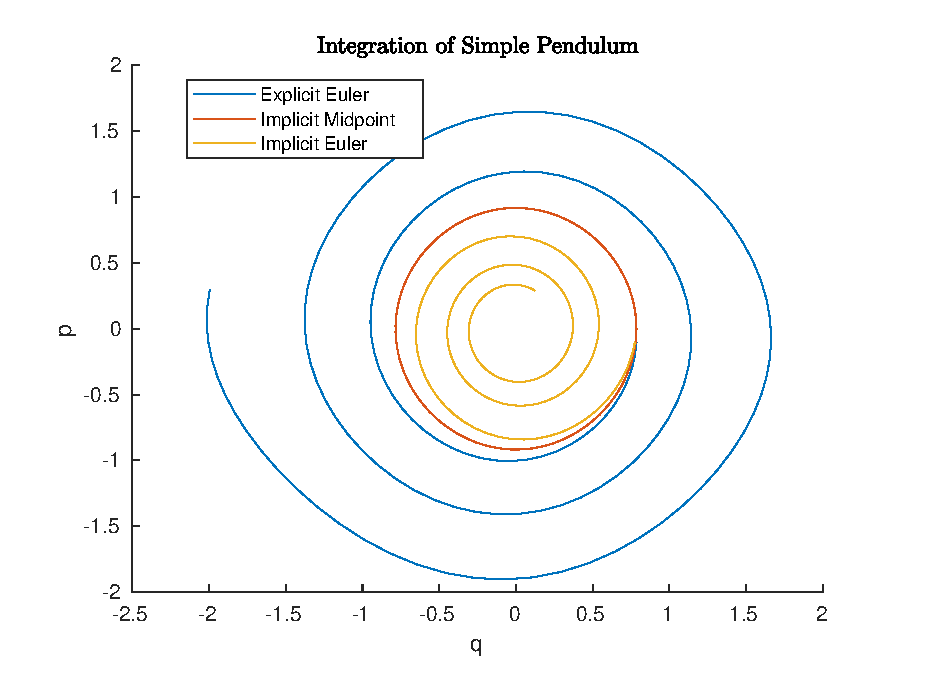
\includegraphics[width=0.75\linewidth]{figures/pendulum.eps}
	\caption{
		Integration of the simple pendulum as a Hamiltonian mechanics problem, plotted as a phase portrait.
		The explicit Euler method gradually diverges, a consequence of it lacking A-stability.
		The implicit Euler method converges to zero.
		Using implicit midpoint, we stay on the path followed by the pendulum, since this method is symplectic.
	}
	\label{fig:pendulum}
\end{figure}

The simple pendulum is the one-dimensional system defined by
\begin{equation*}
	ml\frac{\mathrm{d}^2 \theta}{\mathrm{d}t^2} = - mg \sin(\theta)'
\end{equation*}
For this problem, we define $q = \theta$, $p = \dot{\theta}$ and the Hamiltonian
\begin{equation*}
	H(q,p) = \frac{1}{2}p^2 + k^2(1-\cos(q))
\end{equation*}
where $k^2 = g/l$.
This Hamiltonian can be obtained by integrating the system, and is therefore a conserved quantity.
We will look at a selection of numerical methods applied to this problem.
Recall Euler's method, which takes the form $x_{n+1} = x_n + h \mathbf{J} \nabla H(x_n)$ for a Hamiltonian system.
This expands to:
\begin{equation*}
	\begin{pmatrix}
		q_{n+1} \\
		p_{n+1}
	\end{pmatrix}^E = \begin{pmatrix}
		q_n \\
		p_n
	\end{pmatrix} + h \begin{bmatrix}
		0 & 1 \\
		-1 & 0
	\end{bmatrix} \begin{pmatrix}
		k^2 \sin(q_n) \\
		p_n
	\end{pmatrix} = \begin{pmatrix}
		q_n + h p_n \\
		p_n - h k^2 \sin(q_n)
	\end{pmatrix}.
\end{equation*}
The Implicit Midpoint method gives us
\begin{equation*}
	\begin{pmatrix}
		q_{n+1} \\
		p_{n+1}
	\end{pmatrix}^M = \begin{pmatrix}
		q_n \\
		p_n
	\end{pmatrix} + h \begin{bmatrix}
		0 & 1 \\
		-1 & 0
	\end{bmatrix} \begin{pmatrix}
		k^2 \sin \left(\dfrac{q_n + q_{n+1}}{2}\right) \\
		\dfrac{p_n + p_{n+1}}{2}
	\end{pmatrix} = \begin{pmatrix}
		q_n + h \left( \dfrac{p_n + p_{n+1}}{2} \right) \\
		p_n - h k^2 \sin \left( \frac{q_n + q_{n+1}}{2} \right)
	\end{pmatrix}.
\end{equation*}
Finally, applying the Symplectic Euler-VT method yields
\begin{equation}
	\begin{pmatrix}
		q_{n+1} \\
		p_{n+1}
	\end{pmatrix}^S = \begin{pmatrix}
		q_n \\
		p_n
	\end{pmatrix} + h \begin{bmatrix}
		0 & 1 \\
		-1 & 0
	\end{bmatrix} \begin{pmatrix}
		k^2 \sin(q_n) \\
		p_{n+1}
	\end{pmatrix} = \begin{pmatrix}
		q_n + h p_{n+1} \\
		p_n - h k^2 \sin(q_n)
	\end{pmatrix}
\end{equation}
% change this since the figure uses implicit and explicit Euler and not symplectic euler.

See Figure \ref{fig:pendulum}, where we have applied three methods to the simple pendulum problem.
Only when applying the implicit midpoint method do the oscillations remain on a loop in the phase portrait.
The Symplectic Euler method is not shown, since it is identical to the result obtained from the implicit midpoint method.
The implicit midpoint method is a symplectic method, and probably the simplest to demonstrate.

Symplectic methods preserve the oscillation of the pendulum.
This means the pendulum oscillates consistently, always returning to exactly the same point.
In the explicit and implicit Euler methods, we observe a divergence or convergence of the bounds of oscillation respectively.
% not rigorous, ideally we prove that these methods are symplectic

It is important to note at the moment that the only examples we have looked at have closed form solutions.
Our results so far only serve for understanding the definition of symplecticity.
We now look at some stronger results about numerical methods.

\subsection{The Adjoint Flow Map}

We may now want to look at forming higher order symplectic methods. In order to do so, we need to consider generalised properties of flow maps which define these methods.
One such property is the \textit{adjoint} map.

\begin{definition}
	Given a method defined by a numerical flow $\Psi_h$,
	the adjoint $\Psi^*_h$ is the method that satisfies
	\begin{equation*}
		\Psi^*_{-h} = \Psi^{-1}_h.
	\end{equation*}
\end{definition}

In words, stepping backward with the adjoint method is equivalent to stepping forward with the inverse.
Adjoint methods are very useful. Given an arbitrary method $\Psi_h$,
the method $\Psi_{h/2} \circ \Psi_{h/2}^*$ is symmetric.
A symmetric method is a method that satisfies $\Psi_h^{-1} = \Psi_{-h}$.
This means if we integrate forwards in time by a particular step, and then integrate back,
we return to the original value since we are equivalently applying the inverse.
Time symmetric methods are geometric integrators themselves, preserving time symmetry,
however this is not something we will explore in depth.

We can show that the implicit Euler method is the adjoint of explicit Euler.
First, let $\Psi_h^I$ denote the implicit method and let $\Psi_h^E$ denote the explicit method.
We want to show that $\Psi_h^E = (\Psi_{-h}^I)^{-1}$.
This is equivalent to $\Psi_{-h}^I \circ \Psi_h^E (x) = x$.
If we expand this composition, we obtain
\begin{align*}
	\Phi_{-h}^I \left( \Phi_j^E  (x) \right) &= \Phi_{-h}^I \left( x + h f(x) \right) \\
	&= x + h f(x) - h f\left( \Phi_{-h}^I \left( x + h f(x) \right) \right) \\
	&= x + h f(x) - h f\left( \Phi_{-h}^I \left( \Phi_h^E (x) \right) \right),
\end{align*}
and $\Phi_{-h}^I (\Phi_h^E (x)) = x$ solves this equation. Hence $(\Phi_{-h}^I)^{-1} = \Phi_h^E$.
Note that the explicit and implicit Euler methods cannot be symmetric because they are adjoint.

There are several properties of symplectic methods which may be of interest now.
We have not shown that ($1$) the adjoint of a symplectic method is symplectic, and ($2$) the composition of symplectic methods is symplectic.
These are relatively simple properties which can be proven from the defintions, but it will help our understanding to cover these.
\begin{proposition}
	The adjoint of a symplectic method is symplectic.
\end{proposition}
\begin{proof}
	First of all, the definition of the adjoint method states $\Phi^*_h = \Phi^{-1}_{-h}$.
	By algebraic manipulation,
	\begin{align*}
		\Phi_h^\intercal J \Phi_h &= J \\
		\Rightarrow \Phi_{-h}^\intercal J \Phi_{-h} &= J \\
		\Rightarrow J &= (\Phi_{-h}^{-1})^\intercal J (\Phi_{-h}^{-1}) = (\Phi_h^*)^\intercal J (\Phi_h^*)
	\end{align*}
	and so clearly the adjoint is symplectic.
\end{proof}
This result will be used in tandem with the composition of maps.
\begin{proposition}
	If $\Phi_h$ and $\Psi_h$ are two symplectic maps, then their composition $\Phi_h \circ \Psi_h$ is symplectic.
\end{proposition}
\begin{proof}
	This is done similarly. We have
	\begin{align*}
		\left(\Phi_h \Psi_h\right)^\intercal J \left(\Phi_h \Psi_h\right) &= \Psi_h^\intercal \Phi_h^\intercal J \Phi_h \Psi_h \\
		&= \Psi_h^\intercal J \Psi_h \\
		&= J.
	\end{align*}
	Therefore the composition of symplectic maps is symplectic.	
\end{proof}

We can now introduce a new method using these results.

\subsection{The St\"ormer-Verlet Method}

Earlier, we looked at the Symplectic Euler method, which is a modification of the Euler methods for Hamiltonian integration.
If the Hamiltonian is separable such that $H(q,p) = V(q) + T(p)$, then the Symplectic Euler method is explicit.
This is because in the Symplectic Euler-VT step, we use $p_n$ and $q_n$ to compute $p_{n+1}$, then use $p_{n+1}$ and $q_n$ to compute $q_{n+1}$.
This is exactly the method we applied in our earlier example introducing the Symplectic Euler method.
However, the Symplectic Euler method is generally implicit because a given Hamiltonian for a problem may not be separable.
Denote the Symplectic Euler step by $\Psi_h$. The \textit{St\"ormer-Verlet} method is defined by the step $\Psi_{h/2}^* \circ \Psi_{h/2}$.
Formally, this is
\begin{align*}
	p_{n+\frac{1}{2}} &= p_n - \frac{h}{2}\nabla_q H \left( q_n, p_{n+\frac{1}{2}} \right) \\
	q_{n+1} &= q_n + \frac{h}{2}\left( \nabla_p H \left( q_n, p_{n+\frac{1}{2}} \right) + \nabla_p H \left(q_{n+1}, p_{n+\frac{1}{2}} \right) \right) \\
	p_{n+1} &= p_{n+\frac{1}{2}} - \frac{h}{2} \nabla_q H \left( q_{n+1}, p_{n+\frac{1}{2}} \right).
\end{align*}

\subsection{Mechanics}

% maybe send this bit to appendix
% talk about lagrangian and hamiltonian - canonical conjugate momentum
Before the next example, it helps to define context around the mechanics of Hamiltonian system,
In many cases, a Hamiltonian system has a Hamiltonian $H$ that we can express as $H(q,p) = T(p) + V(q)$.
The Hamiltonian is a conserved quantity of the system, such as the total energy being exchanged.
A \textit{Lagrangian} for a system can be defined as $L(q,p) = T(p) - V(q)$,
a difference in the energies.
The natural conjugate momentum is defined by
\begin{equation}
	p_k := \dfrac{\partial L}{\partial \dot{q}_k}
\end{equation}
for $k = 1,\mathellipsis,n$.
If we have a problem formulated generally, position is usually already defined.
Natural conjugate momentum means we can obtain an expression for momentum which aligns with the properties of Hamiltonian dynamics.
It often helps when defining and solving our own problems for the variables to be defined in this way.

\subsection{A Model for Phonation}

% figure on ODE45 vs a symplectic integrator for this problem, do the mobius-style figure

\begin{figure}
	\centering
	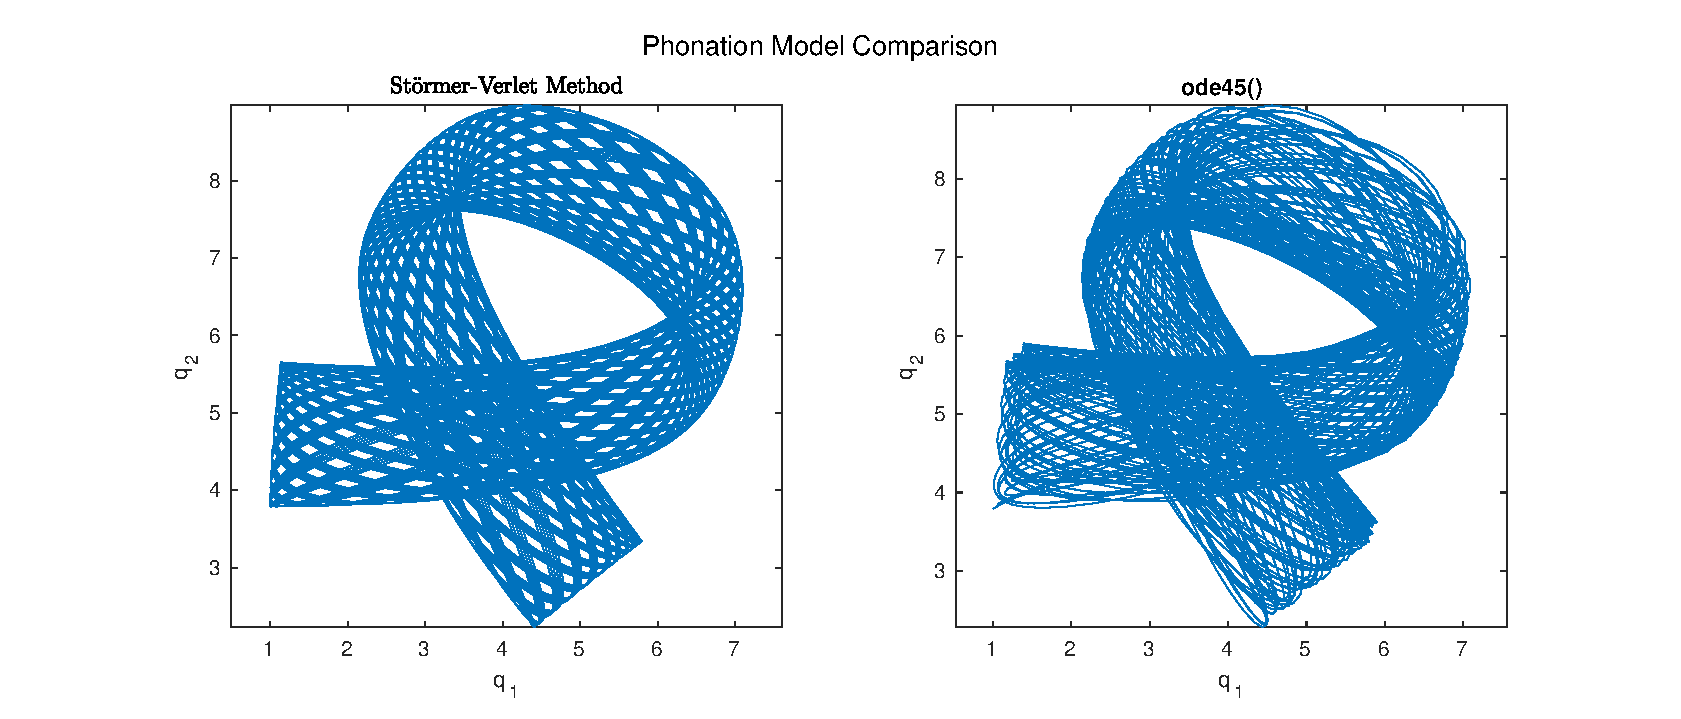
\includegraphics[width = \linewidth]{figures/phonationcomp.eps}
	\caption{
		Integration of the two mass model for phonation for $t \in [0, 1000]$.
		Figures show the oscillation bounds, plotting $q_2$ against $q_1$.
		In the left figure, we observe that a symplectic method retains the bounds of oscillation,
		whereas using \texttt{ode45()} the explicit Runge-Kutta method is not as well behaved and the bounds are not as clear. 
	}
	\label{fig:phon}
\end{figure}

This example is based on the two mass model from ``Models for Phonation''.
A vocal cord is modelled by two stiffness-coupled masses, and their one-dimensional displacements are given by $u$ and $v$.
The governing equation for motion, from Newton's law, is
\begin{align*}
	\dfrac{\mathrm{d}^2 u}{\mathrm{d}t^2} &= 1 - u + \beta \left(1 - \dfrac{1}{u^2}\right) + \omega (v - u) \\
	\alpha \dfrac{\mathrm{d}^2 v}{\mathrm{d}t^2} &= \lambda(1 - v) + \beta \left(1 - \dfrac{1}{v^2}\right) + \omega (u - v) \\
\end{align*}
We first express this as a Hamiltonian problem. Denote $q_1 = u$, $q_2 = v$.
We define momentum $p_1 = \dot{q}_1$, $p_2 = \alpha \dot{q}_2$.
A Hamiltonian, obtained by integrating the system, is
\begin{equation*}
	H = \frac{1}{2} \left( p_1^2 + \frac{1}{\alpha} p_2^2 \right) + \frac{\omega}{2}(q_1 - q_2)^2 - F(q_1) - G(q_2)
\end{equation*}
where
\begin{align*}
	F(q_1) &= q_1 - \frac{1}{2}q_1^2 + \beta \left( q_1 + \frac{1}{q_1} \right) \\
	G(q_2) &= \lambda \left(q_2 - \frac{1}{2}q_2^2 \right) + \beta \left( q_2 + \frac{1}{q_2} \right). \\
\end{align*}
Therefore, in Hamiltonian variables the coupled ODEs can be expressed as
\begin{eqnarray*}
	\dot{q}_1 = p_1 & ~ & \dot{q}_2 = \frac{1}{\alpha} p_2 \\
	\dot{p}_1 = F'(q_1) - \omega(q_1 - q_2) & ~ & \dot{p_2} = G'(q_2) - \omega(q_2 - q_1)
\end{eqnarray*}
stating the problem in Hamiltonian form.
Since the Hamiltonian is a conserved quantity, we can use it to evaluate the behaviour of the integration method.
We can apply the Hamiltonian function to our numerical solutions, to verify that the quantity is in fact conserved by the numerical method.
A symplectic method does not preserve the Hamiltonian, but it preserves a particular Hamiltonian.
The closeness of this Hamiltonian can be shown via backward error analysis.
A regular integration method, such as an explicit Runge-Kutta scheme, will fail to preserve the Hamiltonian and the constant will diverge.
If the value changes by a significant amount, we can observe loss of qualitative behaviour.
Observe how, in Figure \ref{fig:phon}, we have shown an immediate comparison of the clarity of results from using a symplectic integrator,
versus using the efficient but not as stable explicit Runge-Kutta methods applied by MATLAB's \texttt{ode45()} integrator.

\section{Generalised Symplectic Methods}

\subsection{Conjugacy}

Before looking at more symplectic methods, we will cover a brief result on conjugacy of methods.
Consider the implicit midpoint and trapezium methods. Implicit midpoint is the method
\begin{equation*}
	\Phi_h^M (x_n) = x_{n+1} = x_n + hf\left(\frac{x_n + x_{n+1}}{2}\right).
\end{equation*}
The trapezium method is similar:
\begin{equation*}
	\Phi_j^T (x_n) = x_{n+1} = x_n + h \left(\frac{f(x_n) + f(x_{n+1})}{2}\right)
\end{equation*}
The implicit midpoint method is symplectic, but the trapezium method is not.
Interestingly, the trapezium method has excellent behaviour in preserving phase-space volume, despite not being a symplectic method.
It can be shown that these are conjugate methods, meaning that they exhibit similar long-term behaviour.
Two methods $\Psi_h, \Phi_h$ are conjugate if there exists a map $\chi$ such that $\Phi_h = \chi^{-1} \Psi_h \chi$.
Consider applying a method $\Phi_h$ $N$ times. Conjugacy shows that
\begin{align*}
	\left(\Phi_h\right)^N &= \left(\chi^{-1} \Psi_h \chi\right)^N \\
	&= \underbrace{\left(\chi^{-1} \Psi_h \chi \right)\left(\chi^{-1} \Psi_h \chi \right) \mathellipsis \left(\chi^{-1} \Psi_h \chi\right)}_{N} \\
	&= \chi^{-1} (\Psi_h)^N \chi.
\end{align*}
Therefore, conjugate methods remain separated by the conjugacy map $\chi$ for an arbitrary number of iterations.
%% find a defined inverse so that we can show conjugacy.

\subsection{A-Stability}

Show that all symplectic methods must be a-stable.
This justifies that we don't care about any methods that aren't A-stable.

\subsection{Runge-Kutta Methods}

These are methods of the form
\begin{equation*}
	x_{n+1} = x_n + h \left( \sum_{i = 1}^{s} b_i k_i \right)
\end{equation*}
as defined in the introduction, equivalently defined by the Butcher tableau
\begin{equation*}
	\begin{array}{c|ccc}
		c &A \\
		\hline
		&b^\top .
	\end{array}
\end{equation*}
We will first consider A-stability.
In general, the stability function for a Runge-Kutta method \cite{iserles2009rk} is
\begin{equation*}
	r(\lambda) = \frac{\det(I - \lambda A + \lambda eb^\mathrm{T})}{\det(I - \lambda A)}
\end{equation*}
where $A = (a_{ij})$, $b = (b_i)$ and $e$ is the vector of all ones.
The stability function is a rational function in all cases.

Consider the linear test problem $\dot{x} = \lambda x$.
We have already explored stability for the basic Euler methods.
We will look at an explicit 3-stage method.
First, find expressions for the $k_i$:
\begin{align*}
	k_1 &= \lambda x_n, \\
	k_2 &= \lambda\left( x_n + h a_{21}k_1 \right) \\
	&= \left( \lambda + h a_{21}\lambda^2 \right)x_n, \\
	k_3 &= \lambda \left( x_n + h a_{31}k_1 + h a_{32}k_2 \right) \\
	&= \lambda \left( x_n + h a_{31} \lambda x_n + h a_{32}\left( \lambda + h a_{21} \lambda^2 \right) x_n \right) \\
	&= \left( \lambda + h a_{31}\lambda^2 + h a_{32}\lambda^2 + h^2 a_{32}a_{21}\lambda^3 \right) x_n.
\end{align*}
therefore
\begin{align*}
	x_{n+1} &= x_n + h \left( b_1 k_1 + b_2 k_2 + b_3 k_3 \right) \\
	&= x_n + h b_1 \lambda x_n + h b_2 \left(\lambda + h a_{21} \lambda^2\right)x_n + hb_3 \left( \lambda + h a_{31} \lambda^2 + h a_{32} \lambda ^2 + h^2 a_{32} a_{21} \lambda^3\right)x_n \\
	&= \left(
		1 + \left( b_1 + b_2 + b_3 \right) h\lambda + \left(
			b_2 a_{21} + b_3 (a_{31} + a_{32})
		\right)h^2\lambda^2 + \left(
			b_3 a_{32} a_{21}
		\right)h^3\lambda^3
	\right)x_n.
\end{align*}
This coefficient term is a polynomial on $h\lambda$, which we denote by $R(h\lambda)$.
For any explicit $k$-stage Runge-Kutta method the stability function is a polynomial.
To ensure A-stability, we require that $|R(h\lambda)| < 0$ for $h \lambda$ in the left half of the complex plane.
For any explicit method, the stability function is a polynomial.
For any polynomial $p(y)$, we diverge to infinity as $|y| \rightarrow \infty$.
Hence it is impossible for any explicit Runge-Kutta method to be A-stable.

It is impossible for explicit RK methods to be A-stable, because the stability functions are polynomials which diverge to infinity as $|h\lambda| \rightarrow \infty$.
Hence the region of convergence cannot contain the left half-plane.
A general Runge-Kutta method is A-stable if $r(\lambda) < 0$ for all $\lambda < 0$.

\subsection{Symplectic Runge-Kutta Methods}

We have shown that all A-stable Runge-Kutta methods are necessarily implicit.
This is also the case for all symplectic Runge-Kutta methods.

\begin{theorem}
\label{thm:symrk}
If a Runge-Kutta method satisfies
\begin{equation}
	b_i a_{ij} + b_j a_{ji} - b_i b_j = 0
\end{equation}
for all $i, j = 1, \mathellipsis, s$ then it is symplectic.
\end{theorem}
\begin{proof}

This proof is in two parts. First, we want to show that any Runge-Kutta method must satisfy this rule in order to preserve quadratic invariants of the system.
Then, we show that any Runge-Kutta method which preserves these invariants is in fact symplectic.

\textit{Part I:}
Start by considering the recurrence $x_1 = x_0 + h \sum_{j=1}^{s} b_i k_i$ and let $C$ be an arbitrary matrix, in which case we can express a quadratic as
\begin{equation}
	x_1^\intercal C x_1 = x_0^\intercal C x_0 + h \sum_{i=1}^{s} b_i k_i^\intercal C x_0 + h \sum_{j=1}^{s} b_j x_0^\intercal C k_j + h^2 \sum_{i=1}^{s} \sum_{j=1}^{s} b_i b_j k_i^\intercal C k_j
\end{equation} % is the simplification correct?
by expanding. We can make a simplification by writing $k_i = f(X_i) = f\left(x_0 + h \sum_{j=1}^{s}a_{ij}k_j\right)$, which is the definition of the $k_i$ evaluations.
The $f$ is the function which defines the dynamical system.
We work out the expansion:
\begin{align*}
	x_1^\intercal C x_1 &= x_0^\intercal C x_0 + h \sum_{i = 1}^{s} b_i f(X_i)^\intercal C X_i - h \sum_{i=1}^{s}b_i f(X_i)^\intercal C \left( h\sum_{j=1}^{s}a_{ij} k_j \right) \\
	&~ +h \sum_{j = 1}^{s} b_j X_j^\intercal C f(X_j) - h \sum_{j=1}^{s}b_j \left( h\sum_{i=1}^{s}a_{ji} k_i \right) C f(X_j) \\
	&~ + h^2 \sum_{i=1}^{s} \sum_{j-1}^{s} b_i b_j k_i^\intercal C k_j \\
	&= x_0^\intercal C x_0 + h \sum_{i=1}^{s} b_i \left(
		\frac{\mathrm{d}}{\mathrm{d}t} X_i^\intercal C X_i
	\right) + h^2 \sum_{i=1}^{s} \sum_{j=1}^{s} (b_i b_j - b_i a_{ij} - b_j a_{ji})k_i^\intercal C k_j
\end{align*}
Note the application of product rule differentiation, namely that
\begin{equation*}
	X^\intercal C f(X) + f(X)^\intercal C X = \frac{\mathrm{d}}{\mathrm{d}t} (X^\intercal C X)
\end{equation*}
and this quadratic first integral.
% explain why these terms should change
Therefore we require $b_i b_j - b_i a_{ij} - b_j a_{ji} = 0$ in order for the method to preserve quadratic invariants.

\textit{Part II:}
Our dynamical system is defined as $\dot{x} = f(x)$ with the initial condition $x(0) = x_0$.
If we differentiate this problem with respect to $x_0$, we obtain
\begin{equation}
\begin{aligned}
	\frac{\mathrm{d}}{\mathrm{d}t} \varphi'_t(x_0) &= f'(\varphi_t(x_0))\varphi'_t(x_0), \\
	\varphi'_0(x_0) &= I
\end{aligned}
\label{eqn:vari}
\end{equation}
This is a differential equation involving the analytical flow map $\varphi_t(x_0)$.
We will use the result that differentiating with respect to the initial condition and applying a symplectic RK method are commutative:
either way we apply these operations, we end with the same result \cite{gni2006}.
The analytic symplecticity criterion is $\varphi_t^\intercal J \varphi_t = J$, which is a quadratic invariant of the system.
Assuming that $\Psi$ denotes a symplectic RK method, we have $\Psi_n^\intercal J \Psi_n$ as the numerical approximation of the symplecticity constant.
If we apply a symplectic RK method to the original problem, we obtain the numerical flow $\Psi_n$.
Equivalently, if we apply a symplectic RK method to the variational equation \ref{eqn:vari}, we have a numerical sensitivity $\Psi'_n$.
Because the operations are commutative, applying a symplectic RK method to the variational equation respects the symplecticity condition.
This is because this operation has the same result as applying the symplectic RK method first,
and then differentiating with respect to $x_0$.
Therefore, Runge-Kutta methods which preserve quadratic first integrals are symplectic.\end{proof} % this is probably fine

% This is similar to when we looked at demonstrating symplecticity of a regular Hamiltonian system.
% Clearly $\varphi'_0(x_0)^\intercal J \varphi'_0(x_0) = IJI = J$.
% If we differentiate $\varphi'_t(x_0)^\intercal J \varphi'_t(x_0)$ with respect to time, the expression reduces to zero.
% We already showed this when we showed that the flow of a Hamiltonian system is symplectic.
% Therefore, this expression is a first integral of the system.
% Since it is quadratic in $\varphi'_t(x_0)$, it will be conserved by the Runge-Kutta methods which satisfy the property that $b_i b_j - b_i a_{ij} - b_j a_{ji} = 0$.
% Therefore the symplectic identity is a quadratic first integral of the system, and hence these Runge-Kutta methods are symplectic. \end{proof}
% one theorem is that if the method satisfies the implicit criterion then it preserves quadratic integrals
% another result shows that RK methods that preserve quadratic integrals are symplectic

% we can prove the commutativity result if we want to but the proofs are a bit rubbish
% If we solve a dynamical system $\dot{x} = f(x)$ using a symplectic Runge-Kutta method, we get a numerical flow map $\varPhi_h(x_0)$.
% We can differentiate this with respect to the intial condition $x_0$ to obtain a sensitivity of the numerical flow $\varPhi'_h(x_0)$.
% However, this sensitivity matrix is equivalent to the numerical flow map obtained by applying a symplectic Runge-Kutta method to $\frac{\mathrm{d}}{\mathrm{d}t}\varphi'_t(x_0) = f'(\varphi_t(x_0))\varphi'_t(x_0)$,
% which is our dynamical system differentiated with respect to the initial condition. The operations are commutative.
% We will prove this in the following:

% \begin{theorem}
% \label{thm:commt}
% 	For a dynamical system $\dot{x} = f(x)$, applying a symplectic Runge-Kutta method and differentiating the system with respect to $x_0$ are commutative operations.
% 	Regardless of the order in which they are applied, we obtain a numerical flow map $\varPhi'_h(x_0)$ to the dynamical system $\frac{\mathrm{d}}{\mathrm{d}t}\varphi'_t(x_0) = f'(\varphi_t(x_0))\varphi'_t(x_0)$ on the analytical flow map.
% \end{theorem}
% \begin{proof}
% % begin proof
% \end{proof}

% symplectic RK methods preserving quadratic first integrals
% the commutative diagram result

Symplectic Runge-Kutta methods are popular choices for symplectic integration.
We are able to construct symplectic RK methods to a given order, like traditional RK methods.
A known class of symplectic Runge-Kutta methods are Gauss-Legendre Runge-Kutta methods, which satisfy the identity from Theorem \ref{thm:symrk}.
The fourth-order GLRK method is given by the following Butcher tableau:
\begin{equation*}
	\begin{array}{c|cc}
		\frac{1}{2} - \frac{1}{6}\sqrt{3}  &\frac{1}{4} &\frac{1}{4} - \frac{1}{6}\sqrt{3} \\
		\frac{1}{2} + \frac{1}{6}\sqrt{3}  &\frac{1}{4} + \frac{1}{6}\sqrt{3} &\frac{1}{4} \\
		\hline
		&\frac{1}{2} &\frac{1}{2}.
	\end{array}
\end{equation*}
The Gauss-Legendre Runge-Kutta method on two stages is fourth order \cite{iserles2009rk}.
Hence this must be a fourth-order symplectic method.


\subsection{Consideration}

We need implicit runge kutta methods for symplectic runge kutta methods
can we also find conjugate symplectic methods that are easy to compute.


\section{Analysis of Symplectic Methods}

\subsection{Backward Error Analysis}

When we perform numerical integration on a dynamical system given by $\dot{x} = f(x)$,
we obtain a numerical solution in the form of the iteration $x_{n+1} = \Phi_h(x_n)$,
where $\Phi$ is a method of our choice.
This is a numerical solution, which may converge to the exact solution as $h \rightarrow 0$,
but it is not exact.
In backward error analysis, we look at the problem from another perspective.
Instead of considering the closeness of our numerical solution to the system,
we think of the numerical solution as an exact solution to a perturbed problem,
and analyse the perturbation of this new problem to the original.

These methods and theorems follow the methods in Chapter IX of \cite{gni2006}.
We want to find a modified equation $\dot{\tilde{x}} = f_h (\tilde{x})$ which is similar to $\dot{x} = f(x)$,
and which is exactly solved by the obtained numerical solution, i.e, $x_n = \tilde{x}(nh)$.
We expect the perturbed problem to be of the form
\begin{equation*}
	\dot{\tilde{x}} = f_h(\tilde{x}) = f(\tilde{x}) + h f_2(\tilde{x}) + h^2 f_3(\tilde{x}) + \mathellipsis,
\end{equation*}
namely as a polynomial expansion about the original problem. Important to note is that this series is not guaranteed to converge as an infinite sum.
% We require a truncation, which we will explore in detail later.
Instead, we require a truncation of the series,
which we perform by identifying bounds on the functions $f_i$, and truncate such that an infinimum of upper bounds is attained \cite{Casas_2016}.
We want to match this expression to the numerical method such that $\tilde{x}(t+h) \equiv \Phi_h(\tilde{x}(t))$.
Now consider the expansion of the perturbed problem as a Taylor series about a fixed time $t$. Write
\begin{equation*}
	\tilde{x}(t+h) = \tilde{x}(t) + h \dot{\tilde{x}}(t) + \frac{h^2}{2} \ddot{\tilde{x}}(t) + \mathellipsis
\end{equation*}
and recall we have assumed that $\tilde{x}(t) = f_h(\tilde{x})$.
We can use this to expand the first few terms for clarity:
\begin{equation*}
	\begin{aligned}
		\tilde{x}(t+h) = \tilde{x}(t) &+ \left(
			f_h(\tilde{x})
		\right)h \\
		&+ \left(
			f'_h(\tilde{x})f_h(\tilde{x})
		\right)h^2 \\
		&+ \left(
			(f''_h(\tilde{x})+f'_h(\tilde{x}))f'_h(\tilde{x})f_h(\tilde{x})
		\right)h^3 \\
		&+ \mathellipsis
	\end{aligned}
\end{equation*}
However, recall from the defintion of the perturbed problem that $f_h(x)$ is a polynomial on $h$.
Therefore, the terms expand as
\begin{equation*}
	\begin{aligned}
		\tilde{x}(t+h) = \tilde{x}(t) &+ \left(
			f(\tilde{x}) + h f_2(\tilde{x}) + h^2 f_3(\tilde{x}) + \mathellipsis
 		\right)h \\
		&+ \frac{1}{2!}\left(
			(f'(\tilde{x}) + h f'_2(\tilde{x})  + \mathellipsis)
			(f(\tilde{x}) + h f_2(\tilde{x}) + \mathellipsis)
		\right)h^2 \\
		&+ \frac{1}{3!}\left(
			((f''(\tilde{x}) + f'(\tilde{x})) + \mathellipsis)
			(f'(\tilde{x}) + \mathellipsis)
			(f(\tilde{x}) + \mathellipsis)
		\right)h^3 \\
		&+ \mathellipsis
	\end{aligned}.
\end{equation*}
Now consider the numerical method. Assume that it takes the form
\begin{equation*}
	\Phi_h(x) = x + h f(x) + h^2 d_2(x) + h^3 d_3(x) + \mathellipsis
\end{equation*}
where we can find the $d_i$ functions from the defined method. In order to satisfy the eqivalence we want, we match the coefficients of $h$ in $\tilde{x}(t+h)$ and $\Phi_h(\tilde{x}(t))$:
\begin{align*}
	h^0 &: x=x \\
	h^1 &: f(x) = f(x) \\
	h^2 &: d_2(x) = f_2(x) + \frac{1}{2!}f'(x)f(x) \\
	h^3 &: d_3(x) = f_3(x) + \frac{1}{2!}(f'(x)f_2(x) + f'_2(x)f(x)) + \frac{1}{3!}(f''(x)f'(x)f(x) + f'(x)f'(x)f(x)) \\
	& \vdots
\end{align*}
Since we can find the $d_i$ from the definition of the numerical method, and we know $f(x)$ from the definition of the system,
we can rearrange these expressions to find the functions $f_i$ that define the system.
Therefore it is clear that the numerical solution provides a perturbed problem for which it is an exact solution at discrete time points.
Furthermore, if we assume that the given method is $\mathcal{O}(h^p)$,
then we have that $f_i = 0$ for $i \leq p$.
This is because the expansions of $\tilde{x}(t+h)$ and $x(t+h)$ will be the same up to $\mathcal{O}(h^p)$.
% Since we can find the $d_i$ from the numerical method, and $f(x)$ defines the system,
% we can rearrange this problem to find the functions $f_i$ which define the perturbed Hamiltonian system.
% Therefore, the perturbed Hamiltonian which is exactly solved by the numerical solution exists. 

We next want to consider a Hamiltonian system, and the nature of a modified Hamiltonian obtained from a numerical method.

\subsection{The Perturbed Hamiltonian}

\begin{figure}
	\centering
	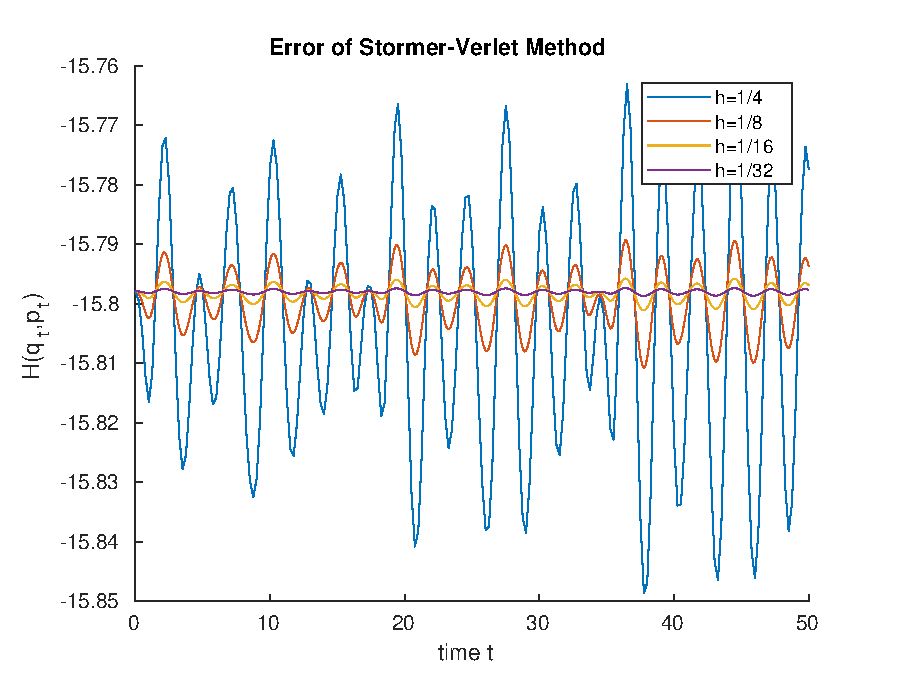
\includegraphics[width = 0.5\linewidth]{figures/phonationerr.eps}
	\caption{
		Evaluating the Hamiltonian for the model for phonation, integrated using the St\"ormer-Verlet method.
		Initial conditions are the same as that of Figure \ref{fig:phon}.
		The error of the method is shown to be $\mathcal{O}(h^2)$ in evaluating the Hamiltonian.
	}
	\label{fig:phonhamil}
\end{figure}

We move on to discuss results on the closeness of the Hamiltonian that corresponds to the problem solved by the numerical method.
This is an interesting result from backward error analysis.
If we can deduce that the modified Hamiltonian is sufficiently close to the original,
this merits the numerical solution in terms of preservation of quality.

Before considering the modified Hamiltonian, we need to introduce the concept of a generating function.
This methodology is covered in \cite{Casas_2016} in a wider analysis.
These are important when considering a change of coordinates.
First, recall Hamilton's equations
\begin{align*}
	&\dot{q}_i = \frac{\partial H}{\partial p_i}, &\dot{p}_i = \frac{- \partial H}{\partial q_i}.
\end{align*}
Define a new coordinate pair $Q_i = Q_i(q,p,t)$ and $P_i = P_i(q,p,t)$.
There must be another Hamiltonian $\tilde{H}$ which describes these transformed coordinates
\begin{align*}
	&\dot{Q}_i = \frac{\partial \tilde{H}}{\partial P_i}, &\dot{P}_i = \frac{- \partial \tilde{H}}{\partial Q_i}.
\end{align*}
This modified Hamiltonian tells us about the behaviour of the solution in this new coordinate system.
The motivation for this transformation is the aim of describing the behaviour of the system in a potentially simpler form using a different coordinate system. %is it?
There is a relation between these coordinates which is given by
\begin{equation}
	\sum_{i=1}^{d} p_i \mathrm{d}q_i - H \mathrm{d}t = \sum_{i=1}^{d} P_i \mathrm{d}Q_i - \tilde{H} \mathrm{d}t + \mathrm{d}F(q,p).
	\label{eqn:genfunc}
\end{equation}
This is an equation involving differential forms $\mathrm{d}q_i, \mathrm{d}t$, etc. but the key takeaway is the relationship involving the expression $\mathrm{d}F$ between coordinate systems.
The relationship between the Hamiltonians themselves is
\begin{equation*}
	\tilde{H}(Q,P,t) = H(q,p,t) + \frac{\partial F}{\partial t}.
\end{equation*}
We call $F$ a generating function. This is because the definition of $F$ can be used to reconstruct the coordinate transformation.
Note also that we wrote $\mathrm{d}F(q,p)$ on the original coordinates above, but if we know the transformation then we can write $F(q,p)$ and $F(Q,P)$ analogously by inverting the transformation.
This is because $F(Q,P) = F(Q(q,p),P(q,p))$.
We now introduce a result on the modified Hamiltonian.

\begin{theorem}[Hairer, Lubich, Wanner 2006]
Consider a generating function for a numerical method $\Phi_h(q,p)$ given by
\begin{equation}
	F(q,P,h) = h F_1(q,P) + h^2 F_2(q,P) + \mathellipsis
	\label{eqn:methodgen}
\end{equation}
where the functions $F_i$ are defined on some domain $D$ which is an open set.
The modified Hamilton's equations are 
\begin{align*}
	&\dot{q}_i = \frac{\partial \tilde{H}}{\partial p_i}, &\dot{p}_i = \frac{- \partial \tilde{H}}{\partial q_i}.
\end{align*}
where the modified Hamiltonian is
\begin{equation}
	\tilde{H}(q,p) = H(q,p) + h H_2(q,p) + h^2 H_3(q,p) + \mathellipsis
	\label{eqn:powerham}	
\end{equation}
where if the method is order $p$, then $H_i = 0$ for $i \leq p$.
The $H_i$ are defined and smooth on $D$.
Therefore, the closeness of the modified Hamiltonian to the original is $\mathcal{O}(h^p)$.
\end{theorem}

If this domain $D$ is the entire space of points $q,P$ then this result is globally defined, but over some restricted domain the result still holds but only locally.
A proof is given in \cite{gni2006}, but the result features in both and \cite{Casas_2016} gives examples.
The proof makes use of mixed-variable generating functions. If we have a generating function $F$ on $(q,P)$,
then
\begin{align*}
	&Q = \frac{\partial F}{\partial P}(q,P), &p = \frac{\partial F}{\partial q}(q,P).
\end{align*}
Furthermore, the proof requires a particular kind of generating function, being the function $\tilde{F}$ obtained from the solution of the Hamilton-Jacobi partial differential equation
\begin{equation*}
	\frac{\partial \tilde{F}}{\partial t}(q,P,t) = \tilde{H} \left(
		P, q + \frac{\partial \tilde{F}}{\partial P}(q,P,t)
	\right)
\end{equation*}
with initial condition $\tilde{S}(q,P,0) = 0$.
This detail is necessary, and more detail is given in \cite{gni2006}.
We now consider the proof for this result.
\begin{proof}
	Let $P,Q$ be the coordinates for the exact solution of the modified equation defined by the perturbed Hamiltonian $\tilde{H}$.
	We first want a generating function $\tilde{F}(q,P,t)$ defining the coordinate transformation.
	It is given (in the text) that if $\tilde{F}$ is a solution to the Hamilton-Jacobi PDE, then it is a unique solution which defines the map
	\begin{align*}
		&Q = q + \frac{\partial \tilde{F}}{\partial P}(q,P,t), &p = P + \frac{\partial \tilde{F}}{\partial q}(q,P,t).
	\end{align*}
	This is an expression involving $t$, and our numerical method is developed using the parameter $h$.
	We want $\tilde{F}$ here to match the expression $F(q,P,h)$ given in the statement of the theorem at $t=h$.
	We can start by considering $\tilde{F}$ as a series expansion around $t=h$, which will take the form
	\begin{equation*}
		\tilde{F}(q,P,t) = t \tilde{F}_1 (q,P,h) + t^2 \tilde{F}_2 (q,P,h) + \mathellipsis
	\end{equation*}
	If we plug this into the Hamilton-Jacobi PDE, we can compare powers of $t$ to obtain expressions for the terms in the series.
	The results come out by Taylor expansion in one dimension since $\tilde{H}$ evaluates at $P$.
	The first few terms are
	\begin{equation}
		\begin{aligned}
			\tilde{F}_1(q,P,h) &= \tilde{H}(q,P) \\
			2 \tilde{F}_2(q,P,h) &= \frac{\partial \tilde{H}}{\partial q}(q,P,h) \cdot \frac{\partial \tilde{F}_1}{\partial P}(q,P,h) \\
			\mathellipsis
		\end{aligned}
		\label{eqn:genh}
	\end{equation}
	The notation on the arguments is not important since these are just functions,
	but we stick with $(q,P)$ for consistency.
	We have expressions for $\tilde{F}_j$ in terms of derivatives of $\tilde{H}$,
	and we also have an expression for $\tilde{H}$ about $H$ in powers of $h$.
	If we let $\tilde{F}_j$ be \textit{another} series of the form
	\begin{equation*}
		\tilde{F}_j(q,P,h) = \tilde{F}_{j1}(q,P) + h \tilde{F}_{j2}(q,P) + h^2\tilde{F}_{j3}(q,P) + \mathellipsis
	\end{equation*}
	then we can use this expansion, and the expansion of $\tilde{H}$ in Equation \ref{eqn:powerham},
	both in powers of $h$,
	and match coefficients by plugging the terms into the entries in Equation \ref{eqn:genh}.
	Trivially, $\tilde{F}_{1k}(q,P) = H_k(q,P)$ from the first entry, so we have the original Hamiltonian plus a series in powers of $h$.
	For $j=2$, we get terms such as
	\begin{align*}
		2 \tilde{F}_{21}(q,P) &= \frac{\partial H}{\partial q}(q,P) \cdot \frac{\partial H}{\partial P}(q,P) \\
		2 \tilde{F}_{22}(q,P) &= \frac{\partial H_2}{\partial q}(q,P) \cdot \frac{\partial H}{\partial P}(q,P) + \frac{\partial H}{\partial q}(q,P) \cdot \frac{\partial H_2}{\partial q}(q,P) \\
		\mathellipsis
	\end{align*}
	In general for $j > 1$ we have that $\tilde{F}_{jk}(q,P)$ is a function depending on derivatives of $H_l$ for $l \leq k$\footnote{
		The book states $l < k$, however equality is attained, for example $\tilde{F}_{22}$ involves derivatives of $H_2$.
	}.
	Finally, recall the purpose of the generating function.
	The function $F(q,P)$ defines the numerical method.
	Therefore $\tilde{F}(q,P,h)$ needs to match $F(q,P,h)$ as defined in Equation \ref{eqn:methodgen}.
	We get the requirements
	\begin{align*}
		F_1(q,P) &= \tilde{F}_{11}(q,P) \\
		F_2(q,P) &= \tilde{F}_{12}(q,P) + \tilde{F}_{21}(q,P) \\
		\mathellipsis
	\end{align*}
	from comparing coefficients of $h$.
	Recall that we have $\tilde{F}_{1k}(q,P) = H_k(q,P)$ from the first row of Equation \ref{eqn:genh}.
	Therefore, the generating expression is a perturbation from the original Hamiltonian and we have
	\begin{equation*}
		F_j(q,P) = H_j(q,P) + \mathcal{D}_j(H_k(q,P))
	\end{equation*}
	where $\mathcal{D}_j$ is some function of derivatives of $H_k$ for $k \leq j$.
	This expression allows us to determine the $H_j$ given a generating function.
	
	Recall the definition of the generating function from Equation \ref{eqn:genfunc}. %logic is bad but it will have to do.
	Assume that the numerical method defined by the generating function $F$ is $\mathcal{O}(h^r)$.
	This generating function $F$ itself is the same order.
	Since we match terms in $F$ and $\tilde{F}$, both are $\mathcal{O}(h^r)$ i.e. the highest order term is $h^{r+1}$.
	Therefore, we must have that $\tilde{F}_{jk} = H_k = 0$ for $k \leq r$.

	Furthermore, since the $F_j$ are defined in terms of $H_j$, they must be defined on the same domain $D$.
\end{proof}

The direct implication is that a higher order method will converge faster to the true \textit{qualitative behaviour}.
Figure \ref{fig:phonhamil} shows the phonation problem from earlier.
We evaluate the Hamiltonian using its closed form expression using the numerical solution generated by the St\"ormer-Verlet scheme.
As we can see, the perturbed Hamiltonian approaches the unmodified Hamiltonian by $\mathcal{O}(h^2)$, the order of the method.

\section{Applications}

\subsection{Example - The Three-Body Problem}

\begin{figure}
	\centering
	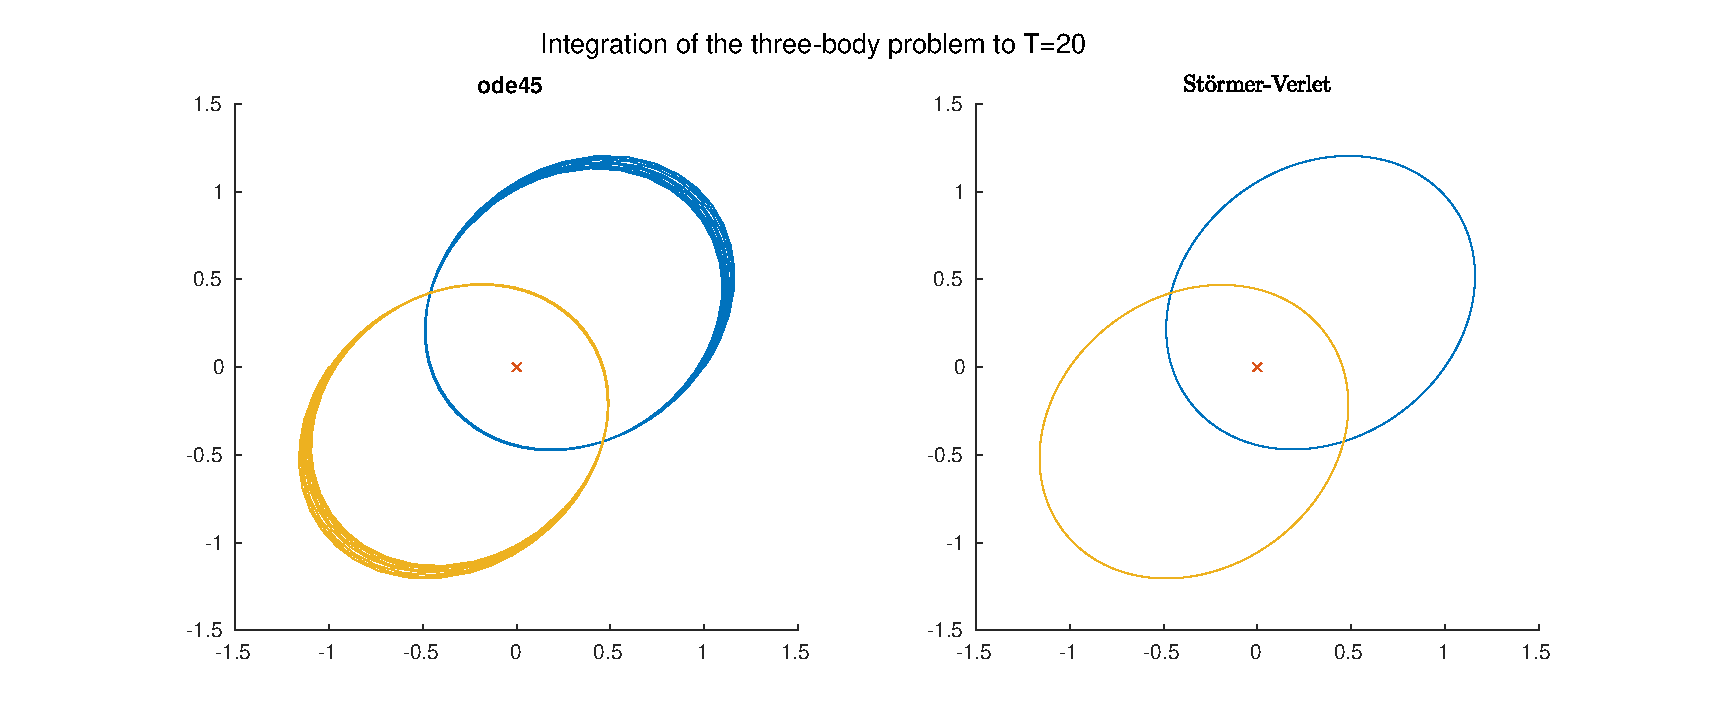
\includegraphics[width=\linewidth]{Matlab/threebodyorbit}
	\caption{
		Integration of the three-body problem for a timespan $t \in [0, 20]$.
		Initial conditions are configured to construct an orbit.
		Two masses orbit a stationary third mass at the origin.
		Initial conditions on the $y=0$ line at $(1,0)$, $(0,0)$ and $(-1,0)$.
		Initial momentum is rotationally symmetric, approximately $(0.35, 0.53)$ at $(1,0)$.
	}
	\label{fig:threebody}
\end{figure}

The three-body problem \cite{musielak2014three} is a huge point of interest in celestial mechanics.
It describes the motion of three point-masses in a closed system which move under gravitational acceleration to each other.
An important subclass is the \textit{restricted} three-body problem, in which one mass is relatively large in magnitude, and can be regarded as fixed compared to the other two bodies.
The restricted three-body problem can be used to model the motion of the earth and moon relative to the sun.

The classical form of the dynamics for the three-body problem is
\begin{equation*}
	\begin{aligned}
		\ddot{x}_1 &= -G m_2 \frac{x_1 - x_2}{|x_1 - x_2|^3} - -G m_3 \frac{x_1 - x_3}{|x_1 - x_3|^3} \\
		\ddot{x}_2 &= -G m_3 \frac{x_2 - x_3}{|x_2 - x_3|^3} - -G m_1 \frac{x_2 - x_1}{|x_2 - x_1|^3} \\
		\ddot{x}_3 &= -G m_1 \frac{x_3 - x_1}{|x_3 - x_1|^3} - -G m_2 \frac{x_3 - x_2}{|x_3 - x_2|^3}
	\end{aligned}
\end{equation*} 
where $x_i$ is the vector position of the point-mass particle with mass $m_i$.
In Hamiltonian form, this is the problem
\begin{align*}
	&\dot{q}_i = \frac{\partial H}{\partial p_i}, &\dot{p}_i = \frac{- \partial H}{\partial q_i}.
\end{align*}
where
\begin{equation*}
	H(q,p) = - \frac{G m_1 m_2}{|q_1 - q_2|} - \frac{G m_2 m_3}{|q_2 - q_3|} - \frac{G m_3 m_1}{|q_3 - q_1|} + \frac{p_1^2}{2m_1} + \frac{p_2^2}{2m_2} + \frac{p_3^2}{2m_3}.
\end{equation*}
for particles with position $q_i$ and momentum $p_i$.

See Figure \ref{fig:threebody} for a visualisation of the trajectories of the three body problem under a particular set of initial conditions.
The integration from \texttt{ode45()} shows clear drift from the original path of the orbit.
A very high relative tolerance of $10^{-12}$ was used for this method, so this is arguably the best approximation we can hope to compute with an explicit method.
In comparison, the St\"ormer-Verlet scheme is only second order accurate, but we are able to maintain the path of orbit over the same timespan because it is a symplectic method.
Any deviation from the orbit path is not visible.

\subsection{Review}

We have given an overview of the structure of problems in Hamiltonian mechanics and how the property of symplecticity is directly related.
We have introduced several symplectic integration methods and the theory behind them.
We have demonstrated these with examples to show the utility of these methods.
It is clear that when the nature of the Hamiltonian is important to the behaviour of the problem, it would be beneficial to use a symplectic method.

Symplectic integration is extremely prevalent in celestial mechanics, where we may need to integrate a Hamiltonian system over a long timespan in order to estimate the motion of celestial bodies far into the future.
The three-body problem is a simple but insightful demonstration of problems such as these.
Other applications in physics are molecular dynamics and particle physics.

Having covered symplectic integration, the theory for which is extremely prevalent and researched,
we now move on to the field of positivity preservation, which is a much more recent and unclear area of geometric numerical integration.

% error control on explicit method versus symplectic method - what is the cost



\documentclass{report}

\usepackage{amsmath}
\usepackage{amssymb}
\usepackage{amsthm}


\newtheorem{theorem}{Theorem}[chapter]
\newtheoremstyle{exampstyle}
  {\topsep} % Space above
  {\topsep} % Space below
  {} % Body font
  {} % Indent amount
  {\bfseries} % Theorem head font
  {.} % Punctuation after theorem head
  {.5em} % Space after theorem head
  {} % Theorem head spec (can be left empty, meaning `normal')
\theoremstyle{exampstyle} \newtheorem{example}[theorem]{Example}
\theoremstyle{exampstyle} \newtheorem{remark}[theorem]{Remark}
\theoremstyle{exampstyle} \newtheorem{definition}[theorem]{Definition}
\theoremstyle{exampstyle} \newtheorem{lemma}[theorem]{Lemma}

\usepackage[english]{babel}
\usepackage{csquotes}
\usepackage{graphicx}
\usepackage{verbatim}
\usepackage{listings}
\usepackage{float}
\usepackage{dsfont}
\usepackage[width=6in, height=8in]{geometry}
\usepackage{xcolor}

\usepackage[
backend=biber,
natbib=true,
url=false, 
doi=true,
eprint=false
]{biblatex}
\addbibresource{sources.bib}

\definecolor{codegreen}{rgb}{0,0.6,0}
\definecolor{codegray}{rgb}{0.5,0.5,0.5}
\definecolor{codepurple}{rgb}{0.58,0,0.82}
\definecolor{backcolour}{rgb}{0.95,0.95,0.92}

\lstdefinestyle{mystyle}{
	backgroundcolor=\color{backcolour},   
	commentstyle=\color{codegreen},
	keywordstyle=\color{magenta},
	numberstyle=\tiny\color{codegray},
	stringstyle=\color{codepurple},
	basicstyle=\ttfamily\footnotesize,
	breakatwhitespace=false,         
	breaklines=true,                 
	captionpos=b,                    
	keepspaces=true,                 
	numbers=left,                    
	numbersep=5pt,                  
	showspaces=false,                
	showstringspaces=false,
	showtabs=false,                  
	tabsize=2
}

\lstset{style=mystyle}

\begin{document}



\chapter{Positivity Preservation}

\section{Positive Solutions to ODEs}

\subsection{Motivation}

There are many problems which motivate the need for numerical methods which preserve positivity of the solution.
For example, consider the problem of simulating a chemical reaction.
We start with a finite amout of positive-valued species at the initial stage, and apply some numerical method to produce a result.
Despite being able to apply methods which have high orders of accuracy, traditional methods will not preserve positivity unconditionally.
If our numerical solution indicates that the concentrations of any number of species become negative, then our solution is not qualitatively accurate to a ``true'' solution.

Consider a problem given by $\dot{x} = f(x)$, with the initial condition $x(0) = x_0$.
For a one-dimensional problem, the true solution is positive if, given $x_0 \ge 0$, we have that $x(t) \ge 0$ for $t>0$.
Positivity of the numerical solution can be expressed as the condition that if $x_i \ge 0$ then $x_{i+1} \ge 0$ for all $i = 1, \mathellipsis, N$ timesteps in the computation.
Like always, $x$ may be vector-valued. If $x \in \mathds{R}^d$,
then the condition for positivity of the numerical solution applies element-wise to each component $x_i^{(k)}$ for $k = 1, \mathellipsis, d$.
Importantly, entries \textit{can} be zero. 

Methods which preserve positivity are a current area of research. It is difficult to produce numerical methods which both preserve positivity and maintain high order accuracy.
Moreover, it is very difficult to formulate positivity preserving methods for general problems.
Our approach will be to consider particular cases, where we can reduce the problem $\dot{x} = f(x)$ to a particular form,
and formulate positivity-preserving methods which are effective for these problems.

\subsection{The Graph-Laplacian Matrix}

Before looking at positivity-preserving methods, we will consider problems which themselves must admit positivity-preserving solutions.
The notion of the graph-Laplacian matrix and the methods centered around it are taken from \cite{blanes_pos_2022}.

Our main focus will be on problems that we can write in the form 
\begin{equation*}
    \dot{x} = A(x)x
\end{equation*}
where $A$ is a graph-Laplacian matrix.

\begin{definition}
    A graph-Laplacian matrix $A \in \mathds{R}^{d \times d}$ is a square matrix that satisfies
    \begin{itemize}
        \item $\mathbf{1}^\intercal A = \mathbf{0}^\intercal ~~ \text{(its column sums are zero)}.$
        \item For all $i, j = 1, \mathellipsis, d$ where $i \ne j$ we have $A_{ij} \ge 0$.
        \item For all $i = 1, \mathellipsis, d$ we have $A_{ii} \le 0$
    \end{itemize}
\end{definition}

Note that here, $A$ can depend on $x$. The entries in $A(x)$ can contain entries of $x$ in any fashion, as long as the definition is satisfied.

\begin{example}
    The Robertson reaction, taken from \cite{blanes_pos_2022}, is given by the matrix equation
    \begin{equation*}
        \frac{\mathrm{d}}{\mathrm{d}t}\begin{pmatrix}
            x_1 \\
            x_2 \\
            x_3
        \end{pmatrix} = \begin{bmatrix}
            -0.04 & 10^4 x_3 & 0 \\
            0.04 & -3\times 10^7 x_2 - 10^4 x_3 & 0 \\
            0 & 3 \times 10^7 x_2 & 0
        \end{bmatrix} \begin{pmatrix}
            x_1 \\
            x_2 \\
            x_3
        \end{pmatrix}.
    \end{equation*}
    This is a matrix equation of the form $\dot{x} = A(x)x$, where $A$ is a graph-Laplacian matrix.
    This problem describes a chemical reaction of three species.
\end{example}

The name ``graph-Laplacian'' comes from graph theory, and the definition is not universally agreed upon.
For our needs, we consider a graph-Laplacian matrix for a directional graph to be the in-degree matrix (diagonal) minus the in-degree adjacency matrix (empty diagonal) of the graph.
If a problem admits the reduction to graph-Laplacian form like the above,
we can show that the solution retains positivity.

\begin{theorem}
    Solutions of $\dot{x} = A(x)x$ retain positivity if $A$ is graph-Laplacian.
\end{theorem}
\begin{proof}
    Consider the solution $x(t^*)$ at time $t^*$. Assume that there are indices $k \in \{1,\mathellipsis, d\}$ where all entries $x_k(t^*)$ are zero and the rest are strictly positive.
    Then the $k$-th equation in the matrix system is
    \begin{equation*}
        \dot{x}_k(t^*) = \sum_{l = 1}^{d} A_{kl}(x(t^*))x_l(t^*).
    \end{equation*}
    Entry $A_{kk}$ is negative, but we assumed $x_k(t^*)=0$ so the only contributions to the sum are the $A_{kl}$ and $x_l$ for $l \ne k$.
    Some of the $x_l$ may be zero but all the rest are positive, so we have $\dot{x}_k \ge 0$.
    Note that equality is attained if all the $x_k$ are zero which is the trivial solution. 
    Assume instead that every entry $x_k(t^*)$ is non-zero and hence positive.
    In this case there are no restrictions on the derivative of the $k$-th entry - the $A_{kk}$ term means this derivative can be negative.
    The $x_k$ term can go to zero, but since the derivative is strictly non-negative at zero, we will retain positivity.
\end{proof}

We have shown that the graph-Laplacian form is a suitable structure for problems where we are concerned about positivity preservation.
From now on, for a vector solution $x \in \mathds{R}^d$ we will write $x \ge 0$ to mean that each element $x_k \ge 0$ for $k = 1, \mathellipsis, d$.
Before moving on to numerical methods that preserve positivity of these problems, we will consider a few points of note.

\subsection{Non-autonomous Systems}

Our analysis so far has focused on problems $\dot{x} = A(x)x$, which are autonomous.
Examples in positivity preservation can often be non-autonomous, which we would write as $\dot{x} = A(x,t)x$.
The particular details of problems involving the graph-Laplacian matrix can be easily analogised to the non-autonomous case.
As such, we will usually only consider problems in the autonomous form, unless it is necessary to the analysis.

Some problems can involve several different timescales,
in which case time-dependence is very important to account for.

\subsection{Conservation of Mass}

%% how graph laplacians also maintain conservation of mass and why this is nice.

When problems describe an exchange of matter, it is useful for this matter to be conserved in our solution.
Conservation of mass is the condition that $x$ satisfies $\mathbf{1}^\top x = C$ for some constant $C$.
Mass is conserved for graph-Laplacian problems because
\begin{equation*}
    \frac{\mathrm{d}}{\mathrm{d}t}\mathbf{1}^\top x = \mathbf{1}^\top \dot{x} = \mathbf{1}^\top A(x)x = \mathbf{0}^\top x = 0
\end{equation*}
hence clearly $\mathbf{1}^\top x$ is constant.
In the literature we often have $C=1$ for simplicity,
there is no loss of generality because this can be applied to some scaling of the initial condition such that $\mathbf{1}^\top x_0 = 1$.

Mass preservation can be generalised to higher order problems involving inner products with the variable of interest.
These problems concern conservation of other properties, which we will not explore in depth.

\section{Positivity Preserving Methods}

% maybe leave this bit for later
\subsection{Brute force approach}

Before considering the problem of positivity preserving methods in depth, we will first consider the method which we will refer to as ``fixing''.
We use the forward Euler method $x_{i+1} = x_i + hf(x_i)$, except at every step we perform a fix by considering every entry in $x_i$ and if it is negative, we just set it to zero.
We can write this formally as the method
\begin{align*}
    x_{i+1} &= x_i + h f(x_i) \\
    x_{i+1} &= \mathcal{H}_+(x_{i+1}) 
\end{align*}
where $\mathcal{H}_+$ is the thresholder that sets all negative entries to zero.
This is equivalent to a projection of $x$ to a vector subspace of lower dimension, determined by in which dimensions $x$ is positive.

This method is very cheap, and it preserves positivity, so it seems like an easy choice.
The fixing step to eliminate negative entries can be applied in general to any numerical method.
%discuss a result

Euler's method serves as a useful baseline to demonstrate experimental ideas.
Being a first-order accurate method, it does not serve as an effective choice for general applications.
We will instead look at different approaches to preserving positivity of the numerical solution,
using the graph-Laplacian structure explored earlier.

\subsection{General Solutions}

Consider the problem $\dot{x} = Ax$, with initial condition $x(t=0) = x_0$, with a constant square matrix $A$.
The general solution to this problem is
\begin{equation*}
    x(t) = \mathrm{e}^{tA} x_0
\end{equation*}
where the matrix exponential is analogised from the scalar case
\begin{equation*}
    \mathrm{e}^A = I + A + \frac{1}{2}A^2 + \frac{1}{6}A^3 + \mathellipsis = \sum_{j=0}^{\infty} \frac{A^j}{j!}.
\end{equation*}
We have shown that in the case where $A$ is graph-Laplacian, solutions preserve positivity.

We can't immediately apply this exponential solution to the problem $\dot{x} = A(x)x$ because of the non-linear right hand side, which will lead to a different expansion via. product rule.
To see why, we will demonstrate the expansion. Assume that the solution for the graph-Laplacian problem is $x(t) = \exp(tA(x))x_0$.
Then
\begin{equation*}
    \dot{x} = \frac{\mathrm{d}}{\mathrm{d}t} \left(
        \mathrm{e}^{A(x)t}x_0 
    \right) = \frac{\mathrm{d}}{\mathrm{d}t} \left[
        A(x)t
    \right] \mathrm{e}^{A(x)t}x_0 = \left[
        A(x) + t A'(x) A(x) x
    \right] x
\end{equation*}
which does not satisfy the problem.
Note that this expension involves a derivative of $A(x)$. More on this later.

\subsection{Exponential Euler's Method and Matrix-Vector Taylor Series}

We said that we can't apply the exponential solution $x(t) = \exp(tA)x_0$ to the problem $\dot{x} = A(x)x$.
We will show this by demonstrating what happens if we do. We propose a method of the form
\begin{equation}
    x_{n+1} = \mathrm{e}^{h A(x_n)}x_n.
\end{equation}
This method fixes $A$ for each step. Therefore, one step is equivalently providing the analytical exponential solution to the problem $\dot{x} = A(y)x$,
where $y = x(t=0) = x_n$.
Considering the true solution after a timestep, we want to find an expression for the \textit{truncation error}.
We write $x(t_n) = x_n$ at the current step and look at the difference between $x(t_n + h)$ (the true value) and $x_{n+1}$ (the method).
However, first we need to consider the Taylor expansion on $x(t + h)$
\begin{equation*}
    x(t+h) = x(t) + h \dot{x}(t) + \frac{h^2}{2}\ddot{x}(t) + \mathellipsis
\end{equation*}
which involves derivatives of the nonlinear vector function $A(x)x$
\begin{equation*}
    x(t+h) = x + h A(x)x + \frac{h^2}{2} \left[ A'(x)A(x)xx + A(x)^2  x \right] + \mathcal{O}(h^3)
\end{equation*}
writing $x = x(t)$.
As we can see, this involves derivatives of $A(x)$, and associativity of matrix multiplication breaks.
To clarify, multiplication following from left to right should always perform defined operations.
Derivatives of $A(x)$ are rank-incrementing tensors: since $A \in \mathds{R}^{d \times d}$,
the first derivative is $A'(x) \in \mathds{R}^{d \times d \times d}$.
The $k$-th order derivative satisfies $A^{(k)}(x) \in \mathds{R}^{d^{k+2}}$.
This analysis is essential for deriving the order of methods for problems of the form we are working with.

Evaluating the truncation error of the exponential Euler method gives us the expression
\begin{equation*}
    \begin{aligned}
        \tau(h) = x(t_n + h) - x_{n+1} &= x(t_n + h) - \mathrm{e}^{h A(x_n)}x_n \\
        &= x(t_n) + h \dot{x}(t_n) + \frac{h^2}{2}\ddot{x}(t_n) + \mathcal{O(h^3)} - \mathrm{e}^{h A(x_n)}x_n \\
        &= x_n + h A(x_n)x_n + \frac{h^2}{2}\left( A'(x_n)A(x_n)x_n x_n + A(x_n)^2 x_n \right) + \mathcal{O}(h^3)\\
         &- \left( I + h A(x_n) + \frac{h^2}{2}A(x_n)^2 + \mathcal{O}(h^3) \right)x_n \\
        &= \frac{h^2}{2} \left( A'(x_n) A(x_n) x_n x_n \right) + \mathcal{O}(h^3)
    \end{aligned}
\end{equation*}
hence the exponential Euler method is first order accurate.

\subsection{The Second-Order Strang Splitting Method}

The exponential Euler method involved considering the problem with one fixed component in order to apply the exponential solution.
We will consider the separation of components in more depth as in \cite{blanes_pos_2022} so that we can justify the construction of higher order methods.

We have the problem $\dot{x} = A(x)x$. Introduce the variable $z$ where the initial conditions for $x$ and $z$ satisfy $x(t=0) = x_0 = z_0 = z(t=0)$.
We then write the problem in two parts as
\begin{align*}
    \dot{x} &= A(z)x \\
    \dot{z} &= A(x)z.
\end{align*}
By separating the problem into two, we are essentially solving the problem twice.
However, the way we have distributed $x$ and $z$ means we can decompose this into two separate problems where we solve one for $x$ and one for $z$.
The first problem is
\begin{equation}
    \label{eqn:split1}
    \begin{aligned}
        \dot{x} &= A(z)x \\
        \dot{z} &= 0
    \end{aligned}
\end{equation}
which has solution
\begin{align*}
    x(t) &= \mathrm{e}^{tA(z_0)}x_0 \\
    z(t) &= z_0
\end{align*}
while the second problem is of alternate form for $x$ and $z$
\begin{equation}
    \label{eqn:split2}
    \begin{aligned}
        \dot{x} &= 0 \\
        \dot{z} &= A(x)z
    \end{aligned}
\end{equation}
which has solution
\begin{align*}
    x(t) &= x_0 \\
    z(t) &= \mathrm{e}^{tA(x_0)}z_0.
\end{align*}
It may appear confusing as to why we split the problem into two parts.
We know that if a problem is given by $\dot{x} = A(x)x$ then its solutions preserve positivity.
We also know that if a problem is given instead by $\dot{x} = Ax$ for any constant matrix $A$, then it has general solution given by $x(t) = \exp(tA)x_0$.
Therefore, by splitting the problem into two problems on $x$ and $z$,
the solutions are given by the exponential form since the matrices are fixed in each problem,
and the solutions preserve positivity because the matrices are of graph-Laplacian form.
Therefore these solutions preserve positivity, which we can use to begin constructing methods which maintain this.

The primary method given in \cite{blanes_pos_2022}, which is a solution to Equations \ref{eqn:split1} and \ref{eqn:split2} is given by the 
\begin{equation}
    \begin{aligned}
        x_{n+\frac{1}{2}} &= \exp \left( \frac{h}{2} A(z_n) \right) x_n \\
        z_{n+1} &= \exp \left( h A(x_{n+\frac{1}{2}}) \right) z_n \\
        x_{n+1} &= \exp \left( \frac{h}{2} A(z_{n+1}) \right) x_{n+\frac{1}{2}}.
    \end{aligned}
    \label{eqn:secondorderstrangsplittingmethod}
\end{equation}
The solution $x_n$, $z_n$ or $(x_n + z_n)/2$ is second order accurate. We perform a half step in $x$,
followed by a full step in $z$ and then a second half-step in $x$, similar to Verlet integration.
In \cite{blanes_pos_2022}, it is stated that $|x_n - z_n|$ can be used as an estimate of the truncation error, for the method to be used adaptively with a variable time step. 

%order results from this method
%example comparing some methods
%magnus method

\subsection{Example - A Linear Problem on Two Variables}

\begin{figure}
    \centering
    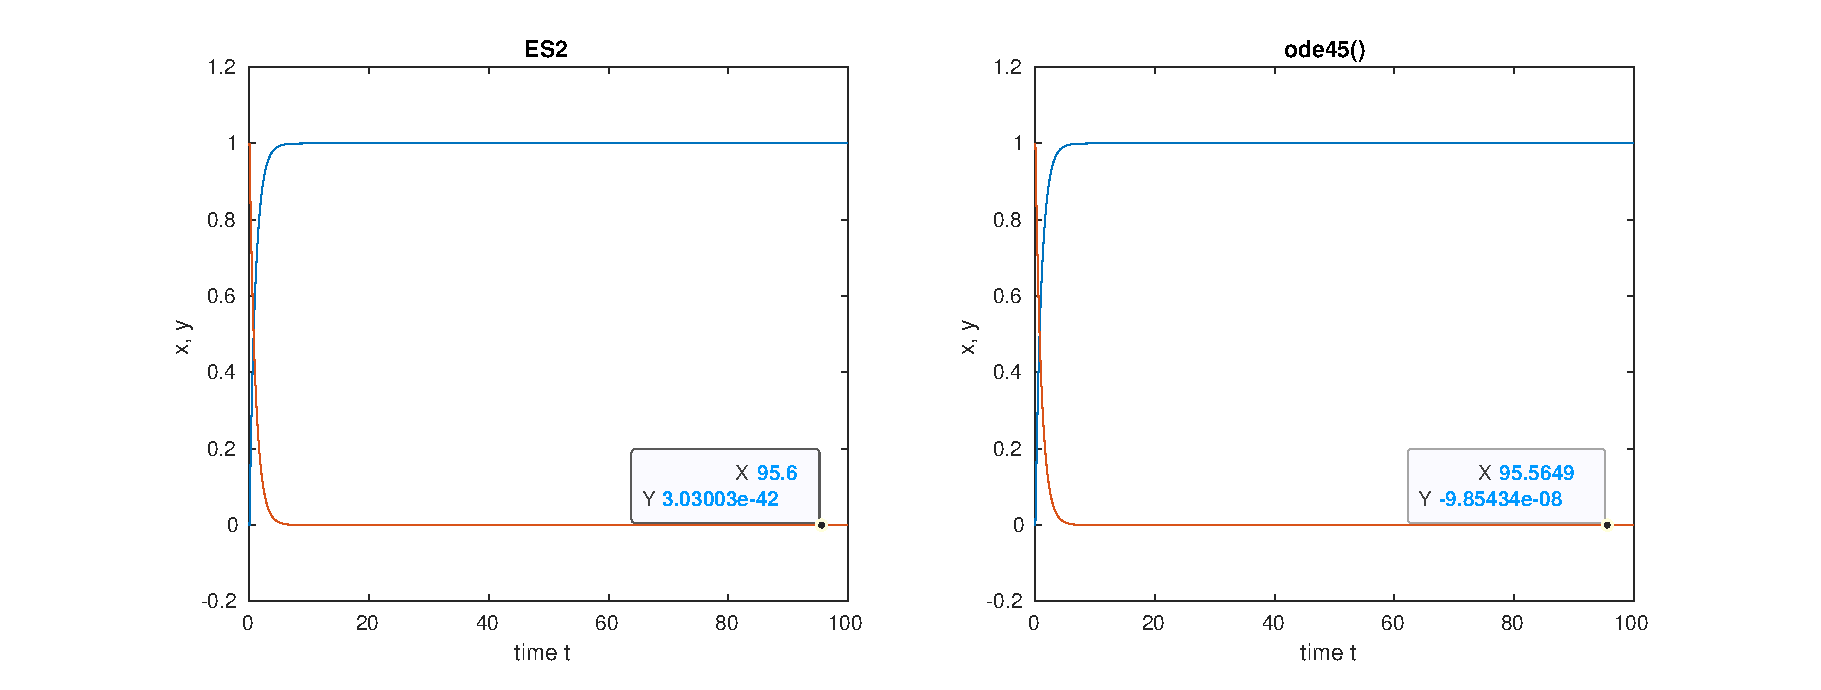
\includegraphics[width = \linewidth]{Matlab/linearproblempositivity.eps}
    \caption{
        Test problem on the system given by Equation \ref{eqn:alineartestproblem}.
        The left figure uses the "ES2" method given by Equation \ref{eqn:secondorderstrangsplittingmethod} taking its $x$ values as opposed to the $z$ values.
        ES2 preserves positivity of the solution throughout.
        The right figure uses MATLAB's \texttt{ode45()} integrator, with a reduced tolerance in order to break positivity.
        The values used were $a=0$ with initial condition $x_0 = 0$, $y_0 = 1$ running for a timespan up to $T = 100$.
        Confusingly the MATLAB graph indexes the horizontal axis $X$ and the vertical $Y$, whereas we plot $x$ and $y$ on the vertical axis against $t$.
        The point labels are necessary to indicate that the MATLAB integrator does not preserve positivity.
    }
    \label{fig:breakposlin}
\end{figure}

Consider the system given by
\begin{equation}
    \frac{\mathrm{d}x}{\mathrm{d}t} = y - ax,~~ \frac{\mathrm{d}y}{\mathrm{d}t} = ax - y
    \label{eqn:alineartestproblem}
\end{equation}
where $a$ is a given constant. This problem is explored briefly for demonstrative purposes in \cite{broekhuizen_biochem_2008}.
The problem admits formulation into the graph-Laplacian form
\begin{equation*}
    \frac{\mathrm{d}}{\mathrm{d}t}\begin{pmatrix}
        x \\
        y
    \end{pmatrix} = \begin{bmatrix}
        -a & 1 \\
        a & -1
    \end{bmatrix} \begin{pmatrix}
        x \\
        y
    \end{pmatrix}
\end{equation*}
where the matrix is constant.

A numerical solution is given in Figure \ref{fig:breakposlin}.
We show that a conventional explicit method, such as the Runge-Kutta method(s) applied in MATLAB's \texttt{ode45()} integrator does not unconditionally preserve positivity.
The formulation of the problem into graph-Laplacian form and the application of a nonnegative initial condition indicates that our solution should preserve positivity, but MATLAB's integrator does not maintain this.
Therefore we have shown that positivity may not be maintained by conventional integrators,
but it is succesful for the ES2 integrator which we know to unconditionally preserve positivity.

\subsection{The Magnus Integrator}

An alternative method suggested in \cite{blanes_pos_2022} is the second order Magnus integrator.
We will first discuss the Magnus expansion \cite{Magnus_1954, blanesmagnus2009}, which allows us to construct this method.
The Magnus expansion considers the linear ODE given by
\begin{equation*}
    \dot{x} = A(t)x
\end{equation*}
with initial condition $x(t=0) = x_0$.
Since $A$ is not time-independent, the exponential solution we have discussed earlier does not hold.
We state that the problem is linear, but the time dependence analogises to the cases we have looked at for a matrix $A(x)$ or $A(t,x)$.
The Magnus expansion considers the solution of this problem to be of the form
\begin{equation*}
    x(t) = \exp(\Omega(t))x_0
\end{equation*}
for some matrix function $\Omega(t)$ which can be expressed in terms of the governing matrix $A$.
We write $\Omega(t)$ as an infinite sum over $\Omega_j(t)$ functions.
From the enclosed sources, we have formulae for these entries.
Specifically, we write
\begin{equation*}
    \begin{aligned}
        \Omega(t) &= \Omega_1(t) + \Omega_2(t) + \mathellipsis = \sum_{j = 0}^{\infty} \Omega_j (t) \\
        \Omega_1(t) &= \int_{0}^{t} A(\tau) \mathrm{d}\tau \\
        \Omega_n(t) &= \sum_{k=1}^{n-1} \frac{B_k}{k!} \int_{0}^{t} S_n^{(j)}(\tau) \mathrm{d}\tau \\
    \end{aligned}
\end{equation*}
where $B_k$ are the Bernoulli numbers \cite{bernoulli} and the $S_n^{(j)}$ functions are defined
\begin{equation*}
    \begin{aligned}
        S_n^{(1)} &= [\Omega_{n-1}, A] \\
        S_n^{(n-1)} &= \operatorname{ad}_{\Omega_1}^{n-1}(A) \\
        S_n^{(j)} &= \sum_{m=1}^{n-j} \left[ \Omega_m, S_{n-m}^{(j-1)} \right] ~~ \text{for}~ 2 \le j \le n-1.
    \end{aligned} 
\end{equation*}
where $\left[\cdot, \cdot\right]$ is the matrix commutator $[A,B] = AB-BA$ and $\operatorname{ad}_A^{j} B = [ A, \operatorname{ad}_A^{(j-1)}B ]$ where $\operatorname{ad}_A^0 B = B$.
We truncate the Magnus expansion to attain an approximation of the solution to a particular order.
Taking just the first term $\Omega_1$, we obtain
\begin{equation*}
    x(t) = \exp\left( \int_{0}^{t} A(\tau) \mathrm{d}\tau \right)x_0
\end{equation*}
which we can approximate with a first order method to get
\begin{equation*}
    x_{n+1} = \exp\left( h A(t) \right)x_n.
\end{equation*}
Note that at a time $\hat{t}$, we can consider $A$ to be a function of $x$ implicitly since $x = x(t)$.
So our previous notions of a problem $\dot{x} = A(x)x$ carry over.
Note also that this first order method is identical to the "exponenial Euler method" we looked at earlier.

The formulation for higher order methods is given in more detail by \cite{blanes_pos_2022} when considering Magnus integrators.
They focus on a second order integrator, for which the autonomous version is given by
\begin{equation}
    x_{n+1} = \exp\left(h A \left( \exp\left(\frac{1}{2}h A(x_n)\right) x_n \right) \right) x_n.
    \label{eqn:secondordermagnus}
\end{equation}
This method uses the midpoint rule in order to form a second order approximation to a formulation of the solution using the first two terms of the Magnus expansion. 

We evaluate the truncation error of the second oder Magnus integrator "EM2", to compare it to our three-exponential "ES2" method.
\begin{equation*}
    \begin{aligned}
        \tau(h) &= x(t_n+h) - \exp \left(
            h A \left( \exp \left(
                \frac{h}{2}A(x_n)
            \right) x_n \right)
        \right) x_n \\
        &= x(t_n + h) - \left(
            I + h A\left(
                \exp \left( \frac{h}{2} A(x_n) \right) x_n
            \right) x_n + \frac{h^2}{2} \left(
                A\left(
                    \exp \left( \frac{h}{2} A(x_n) \right) x_n
                \right)
            \right)^2
        \right) x_n + \mathcal{O}(h^3)
    \end{aligned}
\end{equation*}

% next section is approximating the exponential
\section{Approximating the matrix exponential}
%pade
%the first order approximation
%krylov methods

\subsection{Challenges, series computation}

The positivity preservation methods discussed so far all have one problem in common, being the use of the matrix exponential.
Computing the matrix exponential is significantly expensive, so we hope to introduce some form of approximation by which we can retain a given order of a method.
We might first think to compute the exponential directly from the definition:
\begin{equation*}
    \mathrm{e}^A = I + A + \frac{1}{2}A^2 + \frac{1}{6}A^3 + \mathellipsis = \sum_{j=0}^{\infty} \frac{A^j}{j!}.
\end{equation*}
If we are working in finite precision floating point arithmetic, we can assume that at some point the series will converge such that the sums to $n$ and $n+1$ are represented exactly the same.
In this case, we take the sum to $n$
\begin{equation*}
    \mathrm{e}^A \approx \sum_{j = 0}^{n} \frac{A^j}{j!}.
\end{equation*}
using a modified Horner's form we can express this as
\begin{align*}
	\sum_{j = 0}^{n} \frac{A^j}{j!} &= I + A + \frac{1}{2!}A^2 + \mathellipsis + \frac{1}{n!} A^n \\
	&= I + A\left(
	I + \frac{1}{2} A\left(
			I + \mathellipsis\left(
				\mathellipsis \left( I + \frac{1}{n} A
				\right)
			\right)
		\right)
	\right).
\end{align*}
There are $n$ matrix additions, $n-1$ divisions of a matrix by a scalar and $n-1$ matrix multiplications required to compute this expression.
A multiplication of two $d \times d$ matrices requires $\mathcal{O}(d^3)$\footnote{
    For computer algebra operations, a lower order is better because we often deal with large problems.
    In comparison, we want numerical methods to have higher order because $h$ is often very small.
} floating point operations.
Even with this improvement in efficiency, using this approach to compute a matrix exponential appears expensive.
We will now show that it is also unstable.

The following example is similar to the first demonstration from \cite{moler2003dubious}.
Consider the matrix given by
\begin{equation*}
    A = \begin{bmatrix}
        -121 & 60 \\
        -160 & 79
    \end{bmatrix}.
\end{equation*}
Computing the series form of the exponential directly in double-precision arithmetic sums to $N = 139$ terms, and gives us the solution
\begin{equation*}
    \mathrm{e}_s^A = \begin{bmatrix}
        -2.6531 & -97.1835 \\
        -61.9581 & -184.0359
    \end{bmatrix}.
\end{equation*}
The true form of $A$ can be written as a conjugate transformation
\begin{equation*}
    A = \begin{bmatrix}
        1 & 3 \\
        2 & 4
    \end{bmatrix} \begin{bmatrix}
        -1 & 0 \\
        0 & -41
    \end{bmatrix} \begin{bmatrix}
        1 & 3 \\
        2 & 4
    \end{bmatrix}^{-1}.
\end{equation*}
and so the exponential can be written as 
\begin{equation*}
    e^A = \begin{bmatrix}
        1 & 3 \\
        2 & 4
    \end{bmatrix} \begin{bmatrix}
        \mathrm{e}^{-1} & 0 \\
        0 & \mathrm{e}^{-41}
    \end{bmatrix} \begin{bmatrix}
        1 & 3 \\
        2 & 4
    \end{bmatrix}^{-1} \approx \begin{bmatrix}
        -0.7358 & 0.5518 \\
        -1.4715 & 1.1036
    \end{bmatrix}.
\end{equation*}
Clearly the exponential conputed via series approximation is not an adequate estimate.
% explain the error. moler claims that terms in the sum have magnitudes greater than machine precision of opposite signs, so when adding them we gain terms greater than the final result.

Since this implementation is clearly inadequate, we look for alternative methods for computing the matrix exponential.

\subsection{The Pad\'e Approximation, Scaling and Squaring}

The aim of the Pad\'e approximation for a scalar function $f(x)$ is to construct a rational polynomial approximation to $f$.
The $[n,m]$ Pad\'e approximant for $f$ is the pair $p_{nm}(x), q_{nm}(x)$ which satisfy
\begin{equation*}
    f(x) - \frac{p_{nm}(x)}{q_{nm}(x)} = \mathcal{O}(x^{n+m+1})
\end{equation*} 
where $p_{nm}(x), q_{nm}(x)$ are polynomials.
We generalise this concept to functions on matrices. Given a function $f(A)$, there is a unique $[n,m]$ Pad\'e approximant $R_{mn}(A)$ given by the pair $P_{nm}(A), Q_{nm}(A)$ and formed by $R_{nm}(A) = \left[Q_{nm}(A)\right]^{-1}P_{nm}(A)$
Formulae for Pad\'e approximants for certain matrix functions are known, such as the exponential. 
When computing the product $Q^{-1}P$ we always use a method to solve the system $QX=P$ rather than directly computing the inverse and product.

We said that formulae for the Pad\'e approximation for the exponential are known. From \cite{moler2003dubious} again, we have
\begin{equation}
    \begin{aligned}
        P_{nm}(A) &= \sum_{j=0}^{n} \frac{(n+m-j)!n!}{(n+m)!j!(n-j)!}A^j \\
        Q_{nm}(A) &= \sum_{j=0}^{m} \frac{(n+m-j)!m!}{(n+m)!j!(m=j)!}(-A)^j.
    \end{aligned}
\end{equation}
This is the approximant at zero.
A general Pad\'e approximant is taken about a point, such that it is equal to the approximated function at that point, similar to a Taylor expansion.
In some cases we might take the approximant about a different point, but here zero is no less suitable than anywhere else.

In \cite{blanes_pos_2022} it is stated that the second order diagonal Pad\'e approximation to the exponential is positivity preserving.
This is not true.
This approximation is
\begin{equation*}
    D_{11}(A) = \left[ I - \frac{1}{2}A \right]^{-1} \left[ I + \frac{1}{2} A\right].
\end{equation*}
Consider the matrix given by
\begin{equation*}
    A = \begin{bmatrix}
        -4 & 1 & 0 \\
        2 & -1 & 2 \\
        2 & 0 & -2
    \end{bmatrix}
\end{equation*}
and vector
\begin{equation*}
    x = \begin{bmatrix}
        3 \\
        1 \\
        2
    \end{bmatrix}.
\end{equation*}
To four significant figures the product of the exponential with the vector is
\begin{equation}
    \mathrm{e}^{A} x = \begin{pmatrix}
        0.9422 \\
        3.8506 \\
        1.2071
    \end{pmatrix}
\end{equation}
so positivity is preserved. However if we compute the $[1,1]$ Pad\'e approximant and compute the product we obtain
\begin{equation*}
    \left[D_{11}(A)\right]x = \left[ I - \frac{1}{2}A \right]^{-1} \left[ I + \frac{1}{2}A \right] x = \begin{pmatrix}
        -0.0167 \\
        1.1500 \\
        0.3667
    \end{pmatrix}
\end{equation*}
where we fail to preserve positivity.
A method is proposed in which we exploit the properties of the exponential by writing $A = \bar{A} + \hat{a}I$, such that $\bar{A}$ is entirely nonnegative.
Then
\begin{equation*}
    \mathrm{e}^A = \mathrm{e}^{\bar{A} + \hat{a}I} = \mathrm{e}^{\hat{a}} \mathrm{e}^{\bar{A}}
\end{equation*}
and we compute the $[1,1]$ Pad\'e approximant for $\bar{A}$.
In our example $\hat{a} = -4$ and
\begin{equation*}
    \mathrm{e}^{\hat{a}} [D_{11}(\hat{A})] x = \begin{bmatrix}
        0.5833 \\
        1.7500 \\
       -0.8333
    \end{bmatrix}.
\end{equation*}
So clearly the second order Pad\'e method does not preserve positivity.



\section{Optimisation Methods}

% mass preservation can be recovered from clipping using an optimisation algorithm

% balancing the weights of a RK method - the added constraint enforces positivity


\section{Special Cases}

% the third order method from that chinese paper

% backward Euler





\end{document}

\chapter{Review and Conclusions}

\section{First Section}

\section{Second Section}

Words.

\printbibliography
%give the whole document to overleaf when final compile is needed

\appendix

\chapter{Supplementary Content}

\section{Preliminary}

\subsection{Linear Algebra}

Ascertaining the convergence of computing the matrix exponential requires bounds on matrix norms, particularly in the implementation of scaling and squaring.
There are three vector $p$-norms of interest, where for a vector $x$ we have
\begin{equation*}
    ||x||_p = \left( \sum_{i=1}^{d} x_i^p  \right)^{\frac{1}{p}}.
\end{equation*}
We are only ever concerned with $p=1$ (sum of moduli), $p=2$ (the ``Euclidean norm'') and $p=\infty$ (modulus of maximal element).
Matrix norms are induced by vector norms:
\begin{equation*}
    ||A||_p = \max_x \frac{||Ax||_p}{||x||_p}.
\end{equation*}
The matrix $2$-norm is the most theoretically interesting since it is the spectral radius of the matrix - the modulus of the maximal eigenvalue.
The $1$-norm is the maximum column sum of the moduli of the entries, and the $\infty$ norm is the same for the row sums.
However the norms are equivalent, being that for $p$ and $q$ norms on a matrix $A$ there exist constants $\alpha, \beta$ such that
\begin{equation*}
    \alpha ||A||_q \leq ||A||_p \leq \beta ||A||_q.
\end{equation*}  
Therefore bounds on one norm can be expressed as bounds on any other defined norm.
We use this in the scaling and squaring implementation to avoid computing a matrix $2$-norm \cite{higham2005scaling}.

\subsection{The MATLAB ODE Solvers}

The recommended functions for solving ordinary differential equations in MATLAB are presented as \texttt{odexy()}, where \texttt{x} and \texttt{y} are whole numbers.
These indicate the order of convergence of the methods that they apply in solving the given ODE.
For our purposes, we use \texttt{ode45()}, which uses the Dormand-Prince pair of order $4$ and $5$ explicit Runge-Kutta methods.
The function can be represented in a Butcher tableau
\begin{equation*}
    \begin{array}{c|ccccccc}
		0 \\
        1/5  & 1/5 & & & & & \\
        3/10 & 3/40 &9/40 & & & & \\ 
        4/5  & 44/45 & -56/15 & 32/9 & & & \\
        8/9  & 19372/6561 & -25360/2187 & 64448/6561 & -212/729 & &  \\
        1    & 9017/3168 & -355/33 	& 46732/5247 	& 49/176 	& -5103/18656 & \\
        1  	 & 35/384 	&0 	& 500/1113 	& 125/192 	& -2187/6784 	& 11/84 \\
		\hline
		& 35/384     & 0 & 500/1113   & 125/192 & -2187/6784    & 11/84    & 0 \\
        & 5179/57600 & 0 & 7571/16695 & 393/640 & -92097/339200 & 187/2100 & 1/40.
	\end{array}
\end{equation*}
The first row representing $b^\top$ is the linear combination of the $k_i$ which is fifth-order accurate, while the second row corresponds to the fourth-order method.
The implementation then uses the difference between these methods as an estimate for the error. %cite something

\subsection{The MATLAB Matrix Exponential}

The MATLAB function for computing the matrix exponential employs Pad\'e approximation alongside scaling and squaring.
Given a matrix $A$, a scaling parameter $s$ is chosen such that
\begin{equation*}
    ||A/{2^s}||_\infty < 1/2
\end{equation*}
is satisfied.
The $(6,6)$ Pad\'e approximation of $A/2^s$ is computed and then squared $s$ times.
This approximation is accurate within $\epsilon \approx 10^{-15}$, which is approximately the machine precision for standard double precision $64$-bit arithmetic \cite{moler2003dubious, higham2005scaling}.

\section{Positivity Preservation}

\subsection{Convex Optimisation for ES2}

Denote a vector $g$ of the elements which appear in the expansions of $x(t_n+h)$ and its approximations.
\begin{equation*}
    g := \begin{pmatrix}
        A'' Ax Ax x \\
        A' A' A xxx \\
        A' A^2 xx \\
        A' Ax Ax \\
        A A' A xx \\
        A^3 x
    \end{pmatrix}.
\end{equation*}
We ignore the fact that this is a vector of vectors which is technically not defined.
We denote it as a vector in order to write linear combinations of elements as vector inner products. %dangerous
Define the following vectors
\begin{align*}
    v &:= \begin{pmatrix}
        \frac{1}{6} & \frac{1}{6} & \frac{1}{3} & 0 & \frac{1}{6} & \frac{1}{6}
    \end{pmatrix}^\top \\
    u_z &:= \begin{pmatrix}
        \frac{1}{8} & 0 & \frac{1}{8} & 0 & \frac{1}{4} & \frac{1}{6}
    \end{pmatrix}^\top \\
    u_x &:= \begin{pmatrix}
        0 & \frac{1}{4} & \frac{1}{4} & \frac{3}{8} & \frac{1}{8} & \frac{1}{6}
    \end{pmatrix}^\top .
\end{align*}
Evaluating $v^\top g$ gives us the expansion of the actual value of $x(t_n+h)$ at order $h^3$.
We also have $u_z^\top g$ and $u_x^\top g$, which are the expansions of the $z$ and $x$ components of the method at the same order.
Let $\mu, \lambda$ be scalars for us to take a linear combination of the $x$ and $z$ methods.
The truncation error, denoted here by $\tau$, is
\begin{align*}
    \tau &= v^\top g - \mu ( u_z^\top g ) - \lambda ( u_x^\top g ) \\
    &= \left( v - \mu u_z - \lambda u_x \right)^\top g.
\end{align*}
We aim to optimise this method by minimising the $2$-norm of the vector on the left, since we have control over the parameters $\mu, \lambda$ in our optimisation.
It also serves to note that $g$ is not a vector in the traditional sense and we have no knowledge on the scaling of its entries, therefore it is ignored.
Therefore our problem is of the form
\begin{equation*}
    \text{minimise } ||v - \mu u_z - \lambda u_x||_2.
\end{equation*}
We have the additional contraint that $\mu + \lambda = 1$ in mind, because the method must be second order accurate.
We can block the vectors and scalars to rewrite the problem in the form
\begin{equation*}
    \text{minimise } f(\mu, \lambda) = || v - \begin{bmatrix}
        u_z & u_x
    \end{bmatrix} \begin{pmatrix}
        \mu \\
        \lambda
    \end{pmatrix} ||_2^2.
\end{equation*}
The squared norm makes the computations easier.
If we let this be our objective function, then the constraint function is $g(\mu, \lambda) = (\mu + \lambda - 1)$.
The Lagrangian is
\begin{equation*}
    L(\mu, \lambda, k) = \sum_{i=1}^{6} (v_i - \mu u_{z(i)} - \lambda u_{x(i)})^2 + k (\mu + \lambda - 1)
\end{equation*}
we take partial derivatives of the Lagrangian in order to find the minimiser
\begin{align*}
    \frac{\partial L}{\partial \mu} &= \sum_{i=1}^{6} 2(v_i - \mu u_{z(i)} - \lambda u_{x(i)})(-u_{z(i)}) + k = 2 (\mu u_z^\top u_z + \lambda u_x^\top u_z - v^\top u_z ) + k \\
    \frac{\partial L}{\partial \lambda} &= \sum_{i=1}^{6} 2(v_i - \mu u_{z(i)} - \lambda u_{x(i)})(-u_{x(i)}) + k =  2 (\mu u_z^\top u_x + \lambda u_x^\top u_x - v^\top u_x ) + k \\
    \frac{\partial L}{\partial k} &= \lambda + \mu - 1.
\end{align*}
When all the partial derivatives are zero, this can be written as the linear system
\begin{equation*}
    \begin{bmatrix}
        2u_z^\top u_z & 2u_x^\top u_z & 1 \\
        2u_z^\top u_x & 2u_x^\top u_x & 1 \\
        1 & 1 & 0
    \end{bmatrix} \begin{pmatrix}
        \mu \\
        \lambda \\
        k
    \end{pmatrix} = \begin{pmatrix}
        2v^\top u_z \\
        2v^\top u_x \\
        1
    \end{pmatrix}.
\end{equation*}
We can write this numerically because we know all the values in the vectors, so the system is equivalently
\begin{equation*}
    \begin{bmatrix}
        70 & 52 & 288 \\
        52 & 178 & 288 \\
        288 & 288 & 0
    \end{bmatrix} \begin{pmatrix}
        \mu \\
        \lambda \\
        k
    \end{pmatrix} = \begin{pmatrix}
        76 \\
        100 \\
        288
    \end{pmatrix}
\end{equation*}
having scaled the system to representation in integer values.
The solution is
\begin{align*}
    \mu &= \frac{17}{24} \\
    \lambda &= \frac{7}{24} \\
    k &= \frac{5}{128}.
\end{align*}

% Alternatively we could find a solution to the normal equations.
% Starting with the definition of $f$, the solution to this optimisation problem is the solution to the normal equations
% \begin{equation*}
%     \begin{bmatrix}
%         u_z^\top \\
%         u_x^\top
%     \end{bmatrix} v - \begin{bmatrix}
%         u_z^\top \\
%         u_x^\top
%     \end{bmatrix} \begin{bmatrix}
%         u_z & u_x
%     \end{bmatrix} \begin{pmatrix}
%         \mu \\
%         \lambda
%     \end{pmatrix} = 0.
% \end{equation*}
% which rearranges to
% \begin{equation*}
%     \begin{bmatrix}
%         u_z^\top u_z & u_z^\top u_x \\
%         u_x^\top u_z & u_x^\top u_x
%     \end{bmatrix} \begin{pmatrix}
%         \mu \\
%         \lambda
%     \end{pmatrix} = \begin{bmatrix}
%         u_z^\top v \\
%         u_x^\top v
%     \end{bmatrix}.
% \end{equation*}
% Numerically, this can be represented as
% \begin{equation*}
%     \begin{bmatrix}
%         35 & 26 \\
%         26 & 89
%     \end{bmatrix} \begin{pmatrix}
%         \mu \\
%         \lambda
%     \end{pmatrix} = \begin{bmatrix}
%         38 \\
%         50
%     \end{bmatrix}
% \end{equation*}
% having been scaled up by a factor of $288$.
% Since we must satisfy the linear constraint, we can't directly solve this system.
% With the residual defined as
% \begin{equation*}
%     r = \begin{pmatrix}
%         38 \\
%         50
%     \end{pmatrix} - \begin{bmatrix}
%         35 & 26 \\
%         26 & 89
%     \end{bmatrix} \begin{pmatrix}
%         \mu \\
%         \lambda
%     \end{pmatrix}
% \end{equation*}
% we can write its squared norm as
% \begin{align*}
%     ||r||_2^2 &= \left( 38 - 35 \mu - 26 \lambda \right)^2 + \left( 50 - 26 \mu - 89 \lambda \right)^2 \\
%     &= 1901 \mu^2 + 6448 \mu \lambda + 8597 \lambda^2 - 5260 \mu - 10876 \lambda + 3944
% \end{align*}
% The Lagrangian takes the form $L(\mu, \lambda, k) = ||r||_2^2 + k (\lambda + \mu - 1)$, the objective function plus a Lagrange multiplier $k$ times the constraint function.
% Then
% \begin{align*}
%     \frac{\partial L}{\partial \mu} &= 3802 \mu + 6448 \lambda - 5260 + k \\
%     \frac{\partial L}{\partial \lambda} &= 6448 \mu + 17194 \lambda - 10876 + k \\
%     \frac{\partial L}{\partial k} &= \lambda + \mu - 1.
% \end{align*}
% The minimiser of the Lagrangian is the solution to the linear system
% \begin{equation*}
%     \begin{bmatrix}
%         3802 & 6448 & 1 \\
%         6448 & 17194 & 1 \\
%         1 & 1 & 0
%     \end{bmatrix} \begin{pmatrix}
%         \mu \\
%         \lambda \\
%         k
%     \end{pmatrix} = \begin{pmatrix}
%         5260 \\
%         10876 \\
%         1
%     \end{pmatrix}
% \end{equation*}
% which has the solution
% \begin{align*}
%     \mu &= \frac{19}{30} \\
%     \lambda &= \frac{11}{30} \\
%     k &= \frac{2439}{5}.
% \end{align*}


\chapter{MATLAB Implementations}

Some code is repeated in separate files.

\section{Numerical Integration}

\subsection{Classical Numerical Methods}

\lstinputlisting[language=MATLAB]{Matlab/nummethods.m}


\section{Symplectic Integration}

\subsection{Hamiltonian Methods}
\label{apn:ham}

Three-Body Problem and methods for Hamiltonian framework.
St\"ormer-Verlet integration scheme.

\lstinputlisting[language=MATLAB]{Matlab/sympmethods.m}


\section{Positivity Preservation}

\subsection{Second Order Positivity Preserving Methods}
\label{apn:es2}

ES2 and EM2 applied to the stratospheric reaction model from \cite{blanes_pos_2022}.
Approximations implemented in modifications of ES2.

\lstinputlisting[language=MATLAB]{Matlab/chemexp.m}

\subsection{Testing of Matrix Exponential Approximations}
\label{apn:exp}

\lstinputlisting[language=MATLAB]{Matlab/mypade.m}


\subsection{Second Order Methods IP2, EB2, IQ2}
\label{apn:aprx}

Numerical methods with exponential approximations applied to the MAPK cascade.

\lstinputlisting[language=MATLAB]{Matlab/magnusexperiment.m}












\end{document}